\documentclass[../main.tex]{subfiles}
\begin{document}
\subsection*{Einstein's Postulates}
\begin{quote}
    1. \textbf{The principle of relativity.} The laws of physics apply in all inertial
reference systems.

    2. \textbf{The universal speed of light.} The speed of light in vacuum is the
same for all inertial observers, regardless of the motion of the source.
\end{quote}

\subsection*{Lorentz Transformations}
\textbf{Galilean transformations.} If we “start the clock” ($t = 0$) at the moment the origins ($\mathcal{O}$ and $\bar{\mathcal{O}}$) coincide, then at time $t$, $\bar{\mathcal{O}}$ will be a distance $vt$ from $\mathcal{O}$, and hence
\begin{equation*}
    x=d + vt
\end{equation*}
where d is the distance from $\bar{\mathcal{O}}$ to $\bar{A}$ at time t. Classicaly, $d=\bar{x}$ and thus constructed the Galilean transformations:
\begin{align*}
    \bar{x} &= x - vt\\
    \bar{y} &= y\\
    \bar{z} &= z\\
    \bar{t} &= t
\end{align*}
\begin{figure*}[b]
    \centering
    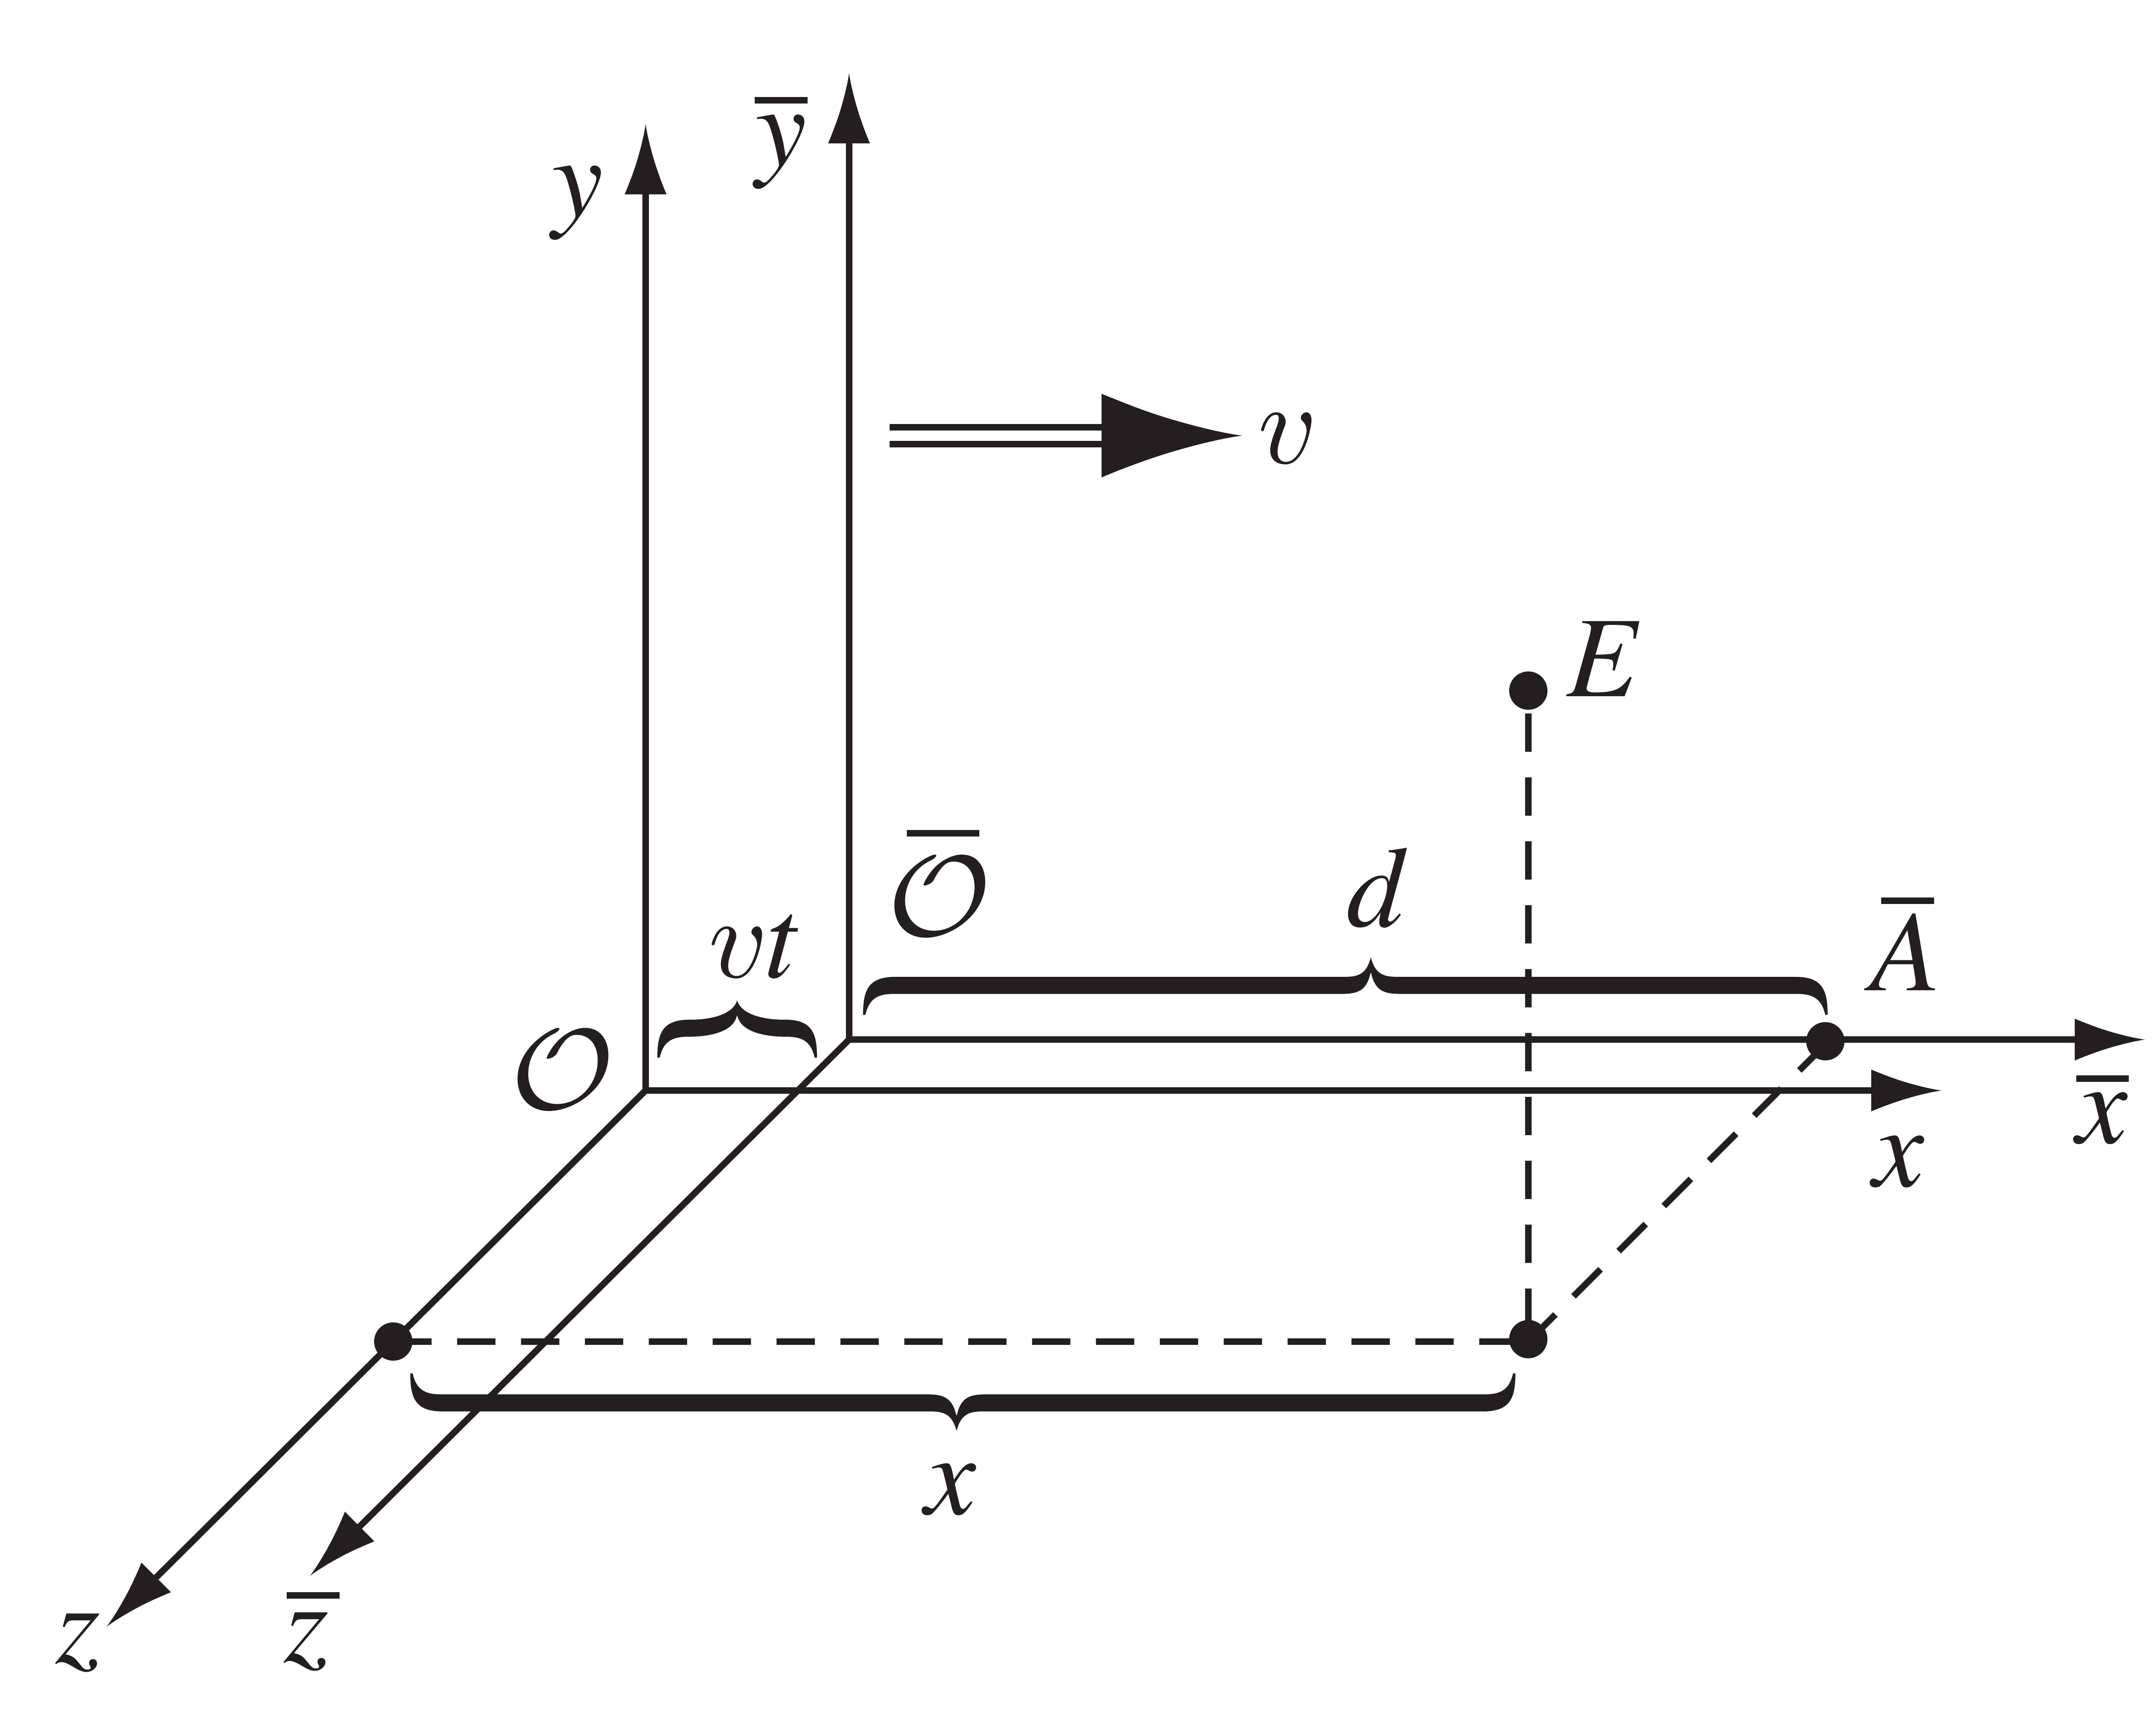
\includegraphics[width=0.45\linewidth]{../Rss/Relativity/Transformation1.png}
    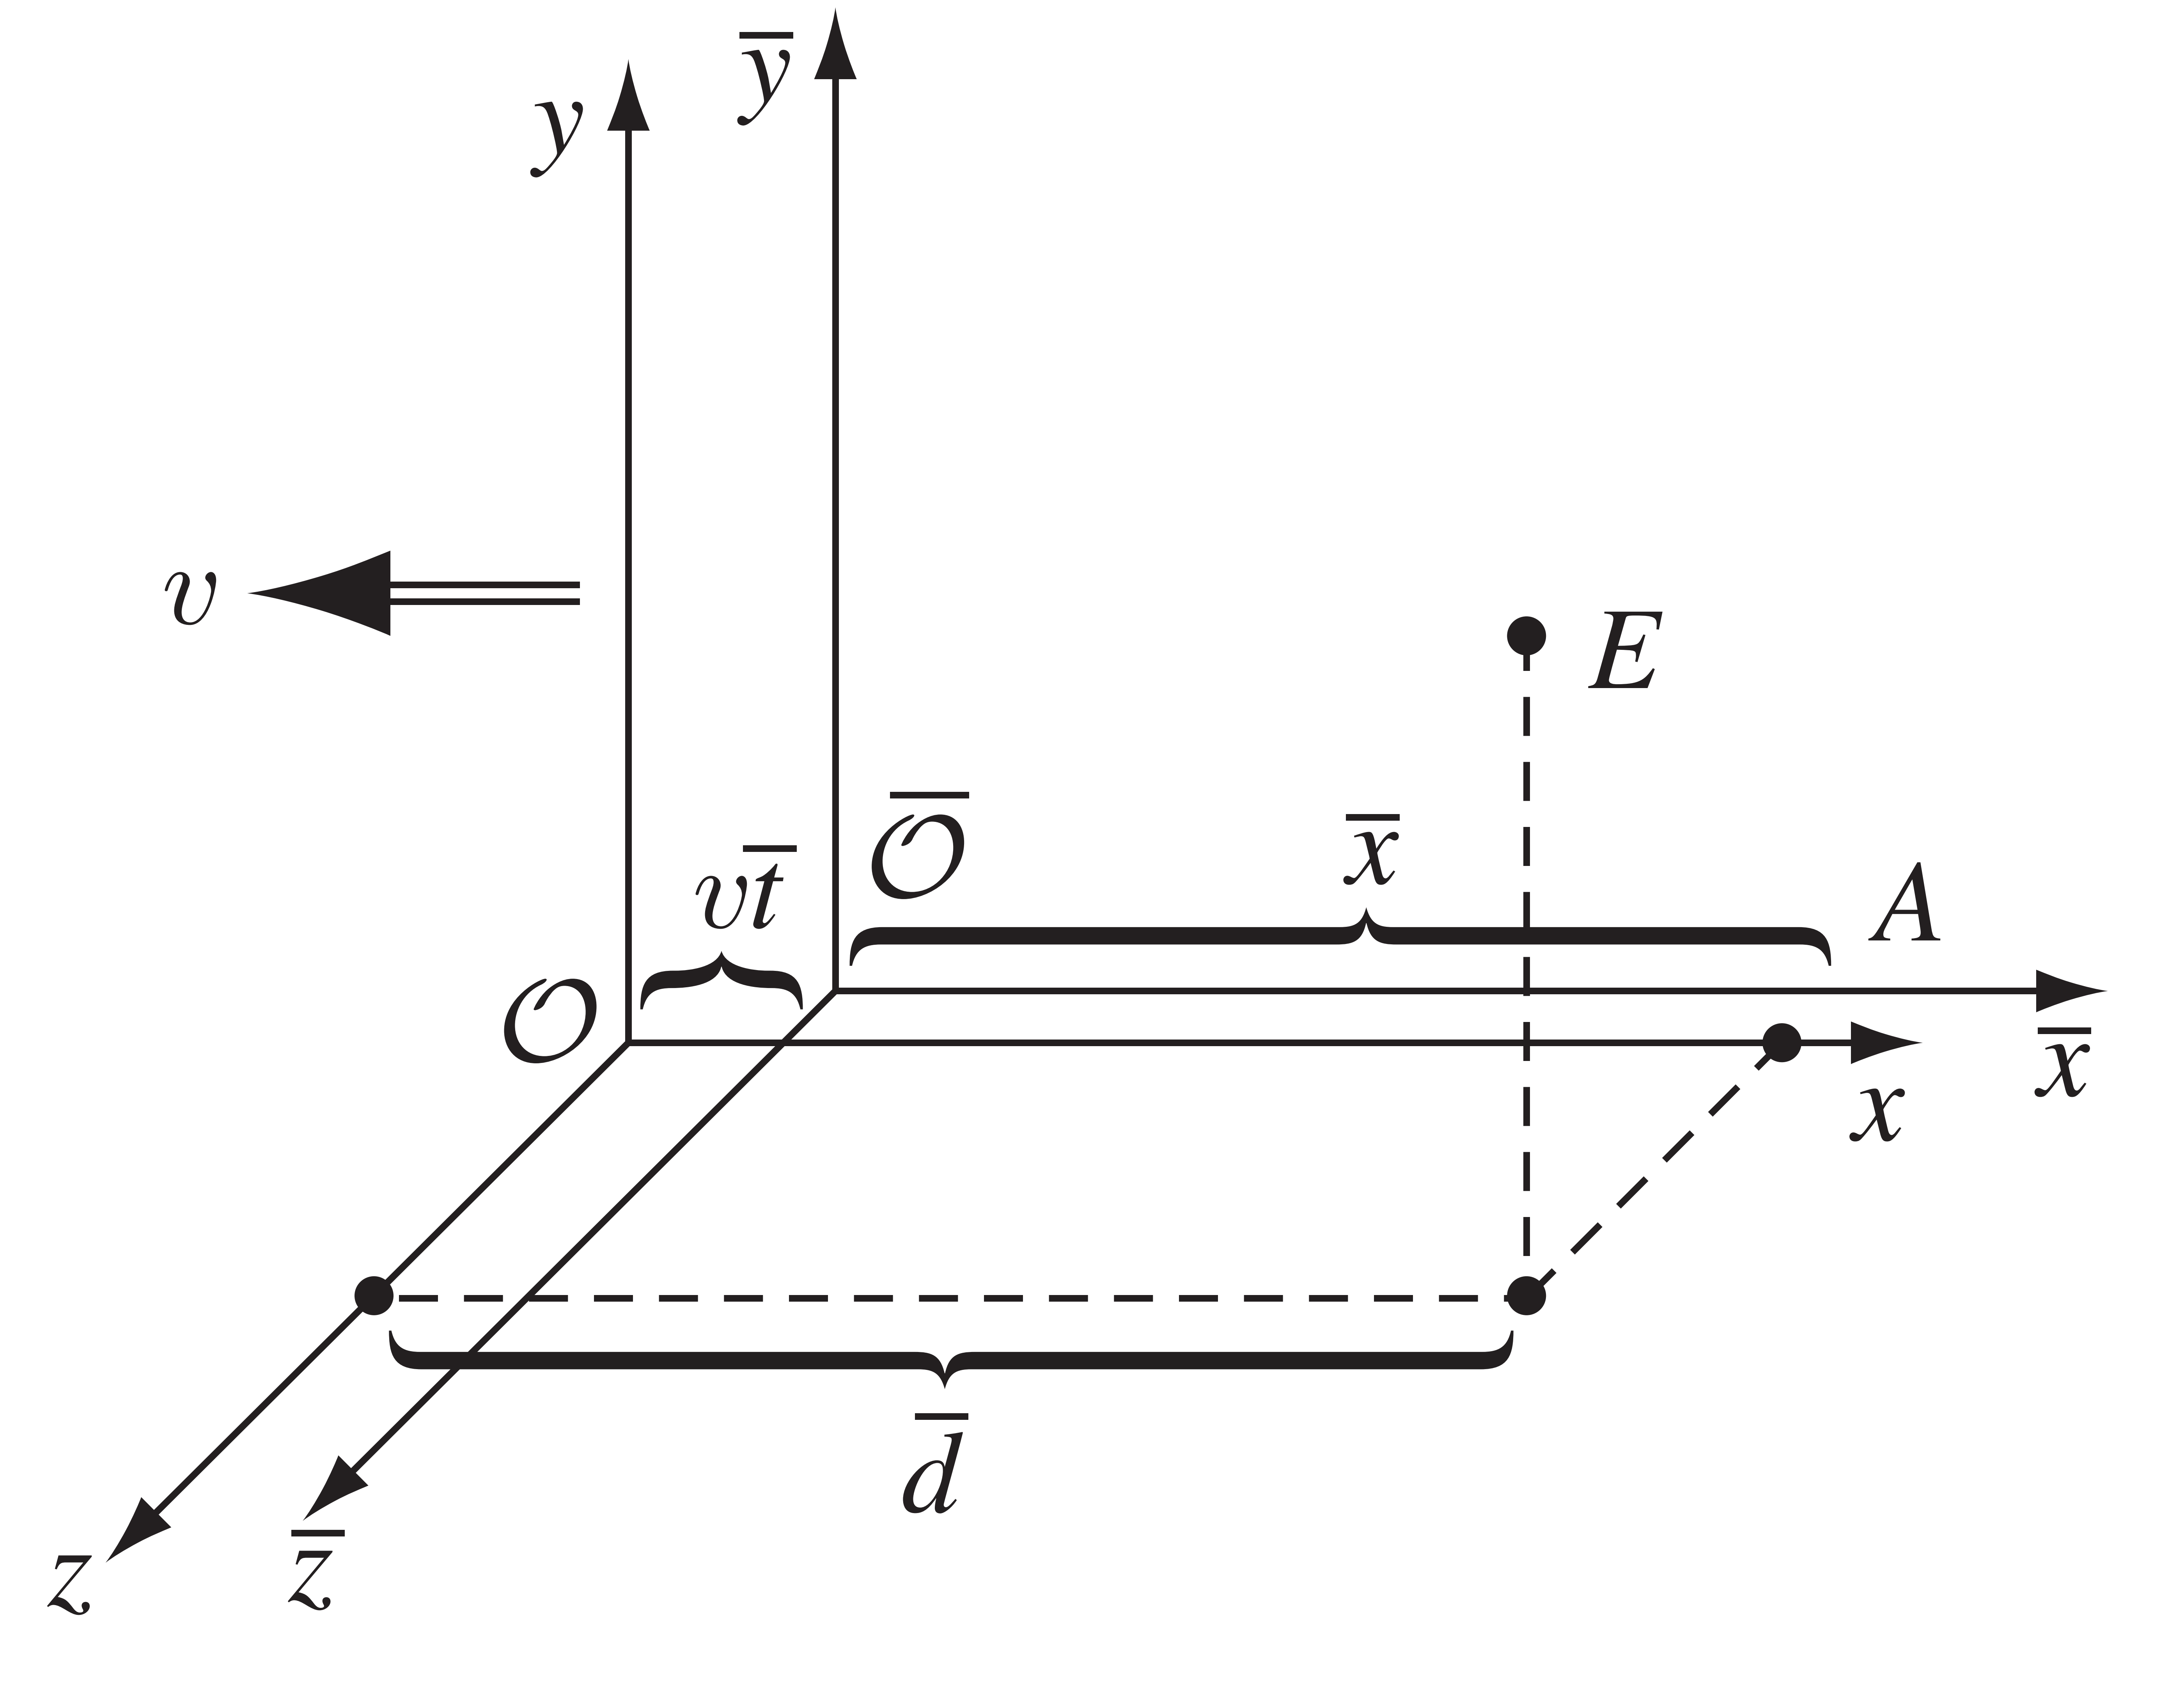
\includegraphics[width=0.45\linewidth]{../Rss/Relativity/Transformation2.png}
    \caption*{Figure: Reminder that in relativity there is no absolute velocity. $\bar{S}$ slides along the $x$ axis at speed $v$ (with $S$ being at rest) is the same as $S$ slides along the $x$ axis at speed $-v$ (with $\bar{S}$ being at rest). Of course that is assuming both systems are inertial.}
\end{figure*}

\textbf{Lorentz transformations.} In relativity, however, there will be a modification for Galilean transformations. As mentioned earlier, d is the distance from $\bar{\mathcal{O}}$ to $\bar{A}$, with the addition that it is meaured by $S$. $ {\mathcal{O}}$ to $\bar{A}$ measured by $\bar{S}$, however, is $\bar{x}$ and is at rest. Therefore
\begin{equation*}
    \bar{x}=\gamma d
\end{equation*}
When this is inserted in Galilean Transformations, we obtain the relativistic version:
\begin{equation*}
    \bar{x} = \gamma (x - vt).
\end{equation*}
Of course, we could have run the same argument from the point of view of $\bar{S}$. The right diagram looks similar, but in this case it depicts the scene at time $\bar{t}$, whereas left diagram showed the scene at time t. If we assume that $\bar{S}$ also starts its clock when the origins coincide, then at time $\bar{t}$, $\mathcal{O}$ will be a distance $v\bar{t}$ from $\bar{\mathcal{O}}$, and therefore
\begin{equation*}
    \bar{x}=\bar{d}-v\bar{t}
\end{equation*}
Similar as before, $\bar{d}$ is the distance from $O$ to $A$ in $\bar{S}$, whereas $x$ is the distance from $\mathcal{O}$ to $A$ in $S$ and is at rest. Therefore
\begin{equation*}
    x=\gamma\bar{d}
\end{equation*}
It follows that
\begin{equation*}
    x=\gamma(\bar{x}+v\bar{t})
\end{equation*}
This last equation obviously be identical to the formula for $\bar{x}$, except for a switch in the sign of v. Nevertheless, this is a useful result, for if we substitute $\bar{x}$, and solve for $\bar{t}$, we complete the relativistic “dictionary”:
\begin{align*}
    \bar{x} &= \gamma (x - vt)\\
    \bar{y} &= y\\
    \bar{z} &= z\\
    \bar{t}&=\gamma\biggl(t-\frac{v}{c^2}x\biggr)
\end{align*}
These are the famous Lorentz transformations. The reverse dictionary, which carries you from $\bar{S}$ back to $S$, can be obtained algebraically by solving for Lorentz transformations x and t, or, more simply, by switching the sign of v:
\begin{align*}
    x &= \gamma (\bar{x}+ v\bar{t})\\
    y &= \bar{y}\\
    z &= \bar{z}\\
    t&=\gamma\biggl(\bar{t}+ \frac{v}{c^2}\bar{x}\biggr)
\end{align*}

\subsection*{Relativity Geometry}
\textbf{The relativity of simultaneity.} Imagine a freight car, traveling at constant speed along a smooth, straight track; someone then switches the lamp on, and the light spreads out in all directions at speed c. The two events in question occur simultaneously. However, to an observer on the ground these same two events are not simultaneous. For the beam going to the back end has a shorter distance to travel than the one going forward. According to this observer, therefore, event (b) happens before event (a). 
\begin{quote}
    Two events that are simultaneous in one inertial system are not, in general, simultaneous in another.
\end{quote}
\begin{figure*}[b]
    \centering
    
\includegraphics[width=\textwidth]{../Rss/Relativity/Simultaneity}
    \caption*{Figure: Train, freight car even}
\end{figure*}
Using Lorentz transformations we could also come to the sam conclusion. Suppose event A occurs at $x_A = 0$, $t_A = 0$, and event B occurs at $x_B = b$, $t_B = 0$. The two events are simultaneous in $S$. But they are not simultaneous in $\bar{S}$, for the Lorentz transformations give $\bar{x}_A = 0$, $\bar{t}_A = 0$ and $\bar{x}_B = \gamma x$, $\bar{t}_b = -\gamma(v/c^2)b$. According $\bar{S}$ then, B occurs before A, as before.

\textbf{Time dilation.} The time it take the light to leaves the bulb and strikes the floor of the car directly below is
\begin{equation*}
    \Delta \bar{t}=\frac{h}{c}
\end{equation*}
\begin{figure*}
    \centering
    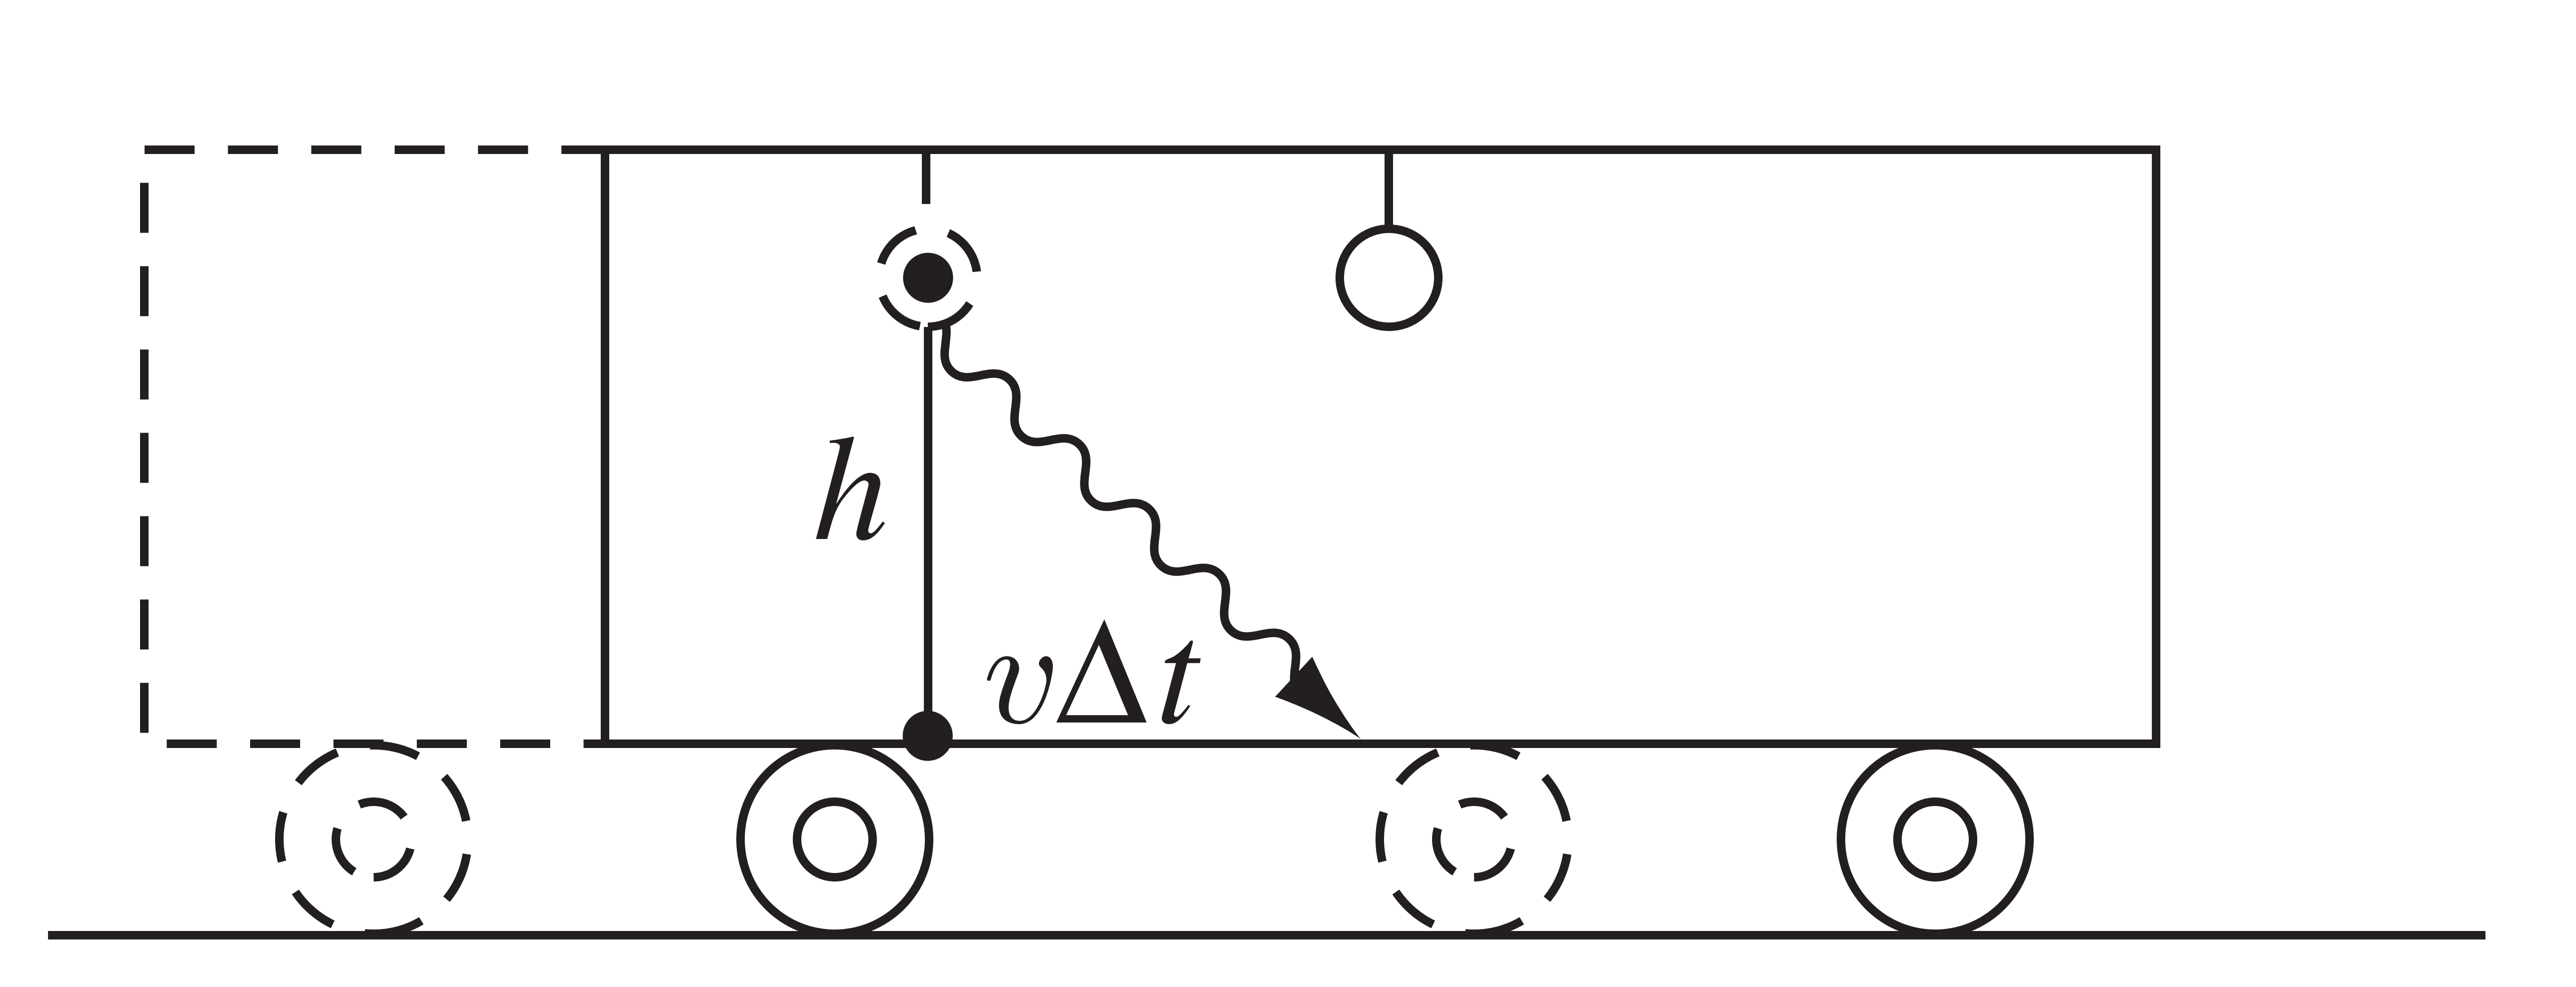
\includegraphics[height=4cm]{../Rss/Relativity/TimeDilatation.png}
    \caption*{How long does it take the light to make this trip?}
\end{figure*}
For an observer, however
\begin{equation*}
    \Delta t=\frac{\sqrt{h^2+(v\Delta t)^2}}{c}
\end{equation*}
Solving for $\Delta t$, we have
\begin{equation*}
    \Delta t=\frac{h}{c}\frac{1}{\sqrt{1-v^2/c^2}}
\end{equation*}
therefore
\begin{align*}
    \Delta \bar{t}&=\sqrt{1-v^2/c^2} \Delta t\\
    &=\frac{1}{\gamma} \Delta t
\end{align*}
This is, by the way, how most textbook introduce constant gamma in relativity. Gamma defined as 
\begin{equation*}
    \gamma\equiv\frac{1}{\sqrt{1-v^2/c^2}}
\end{equation*}

To derive using Lorentz transformations, Suppose that at time $t = 0$ observer $S$ decides to examine all the clocks in $\bar{S}$. He finds that they read different times, depending on their location
\begin{equation*}
    \bar{t}=-\gamma\frac{v}{c^2}x
\end{equation*}
\begin{figure*}
    \centering
    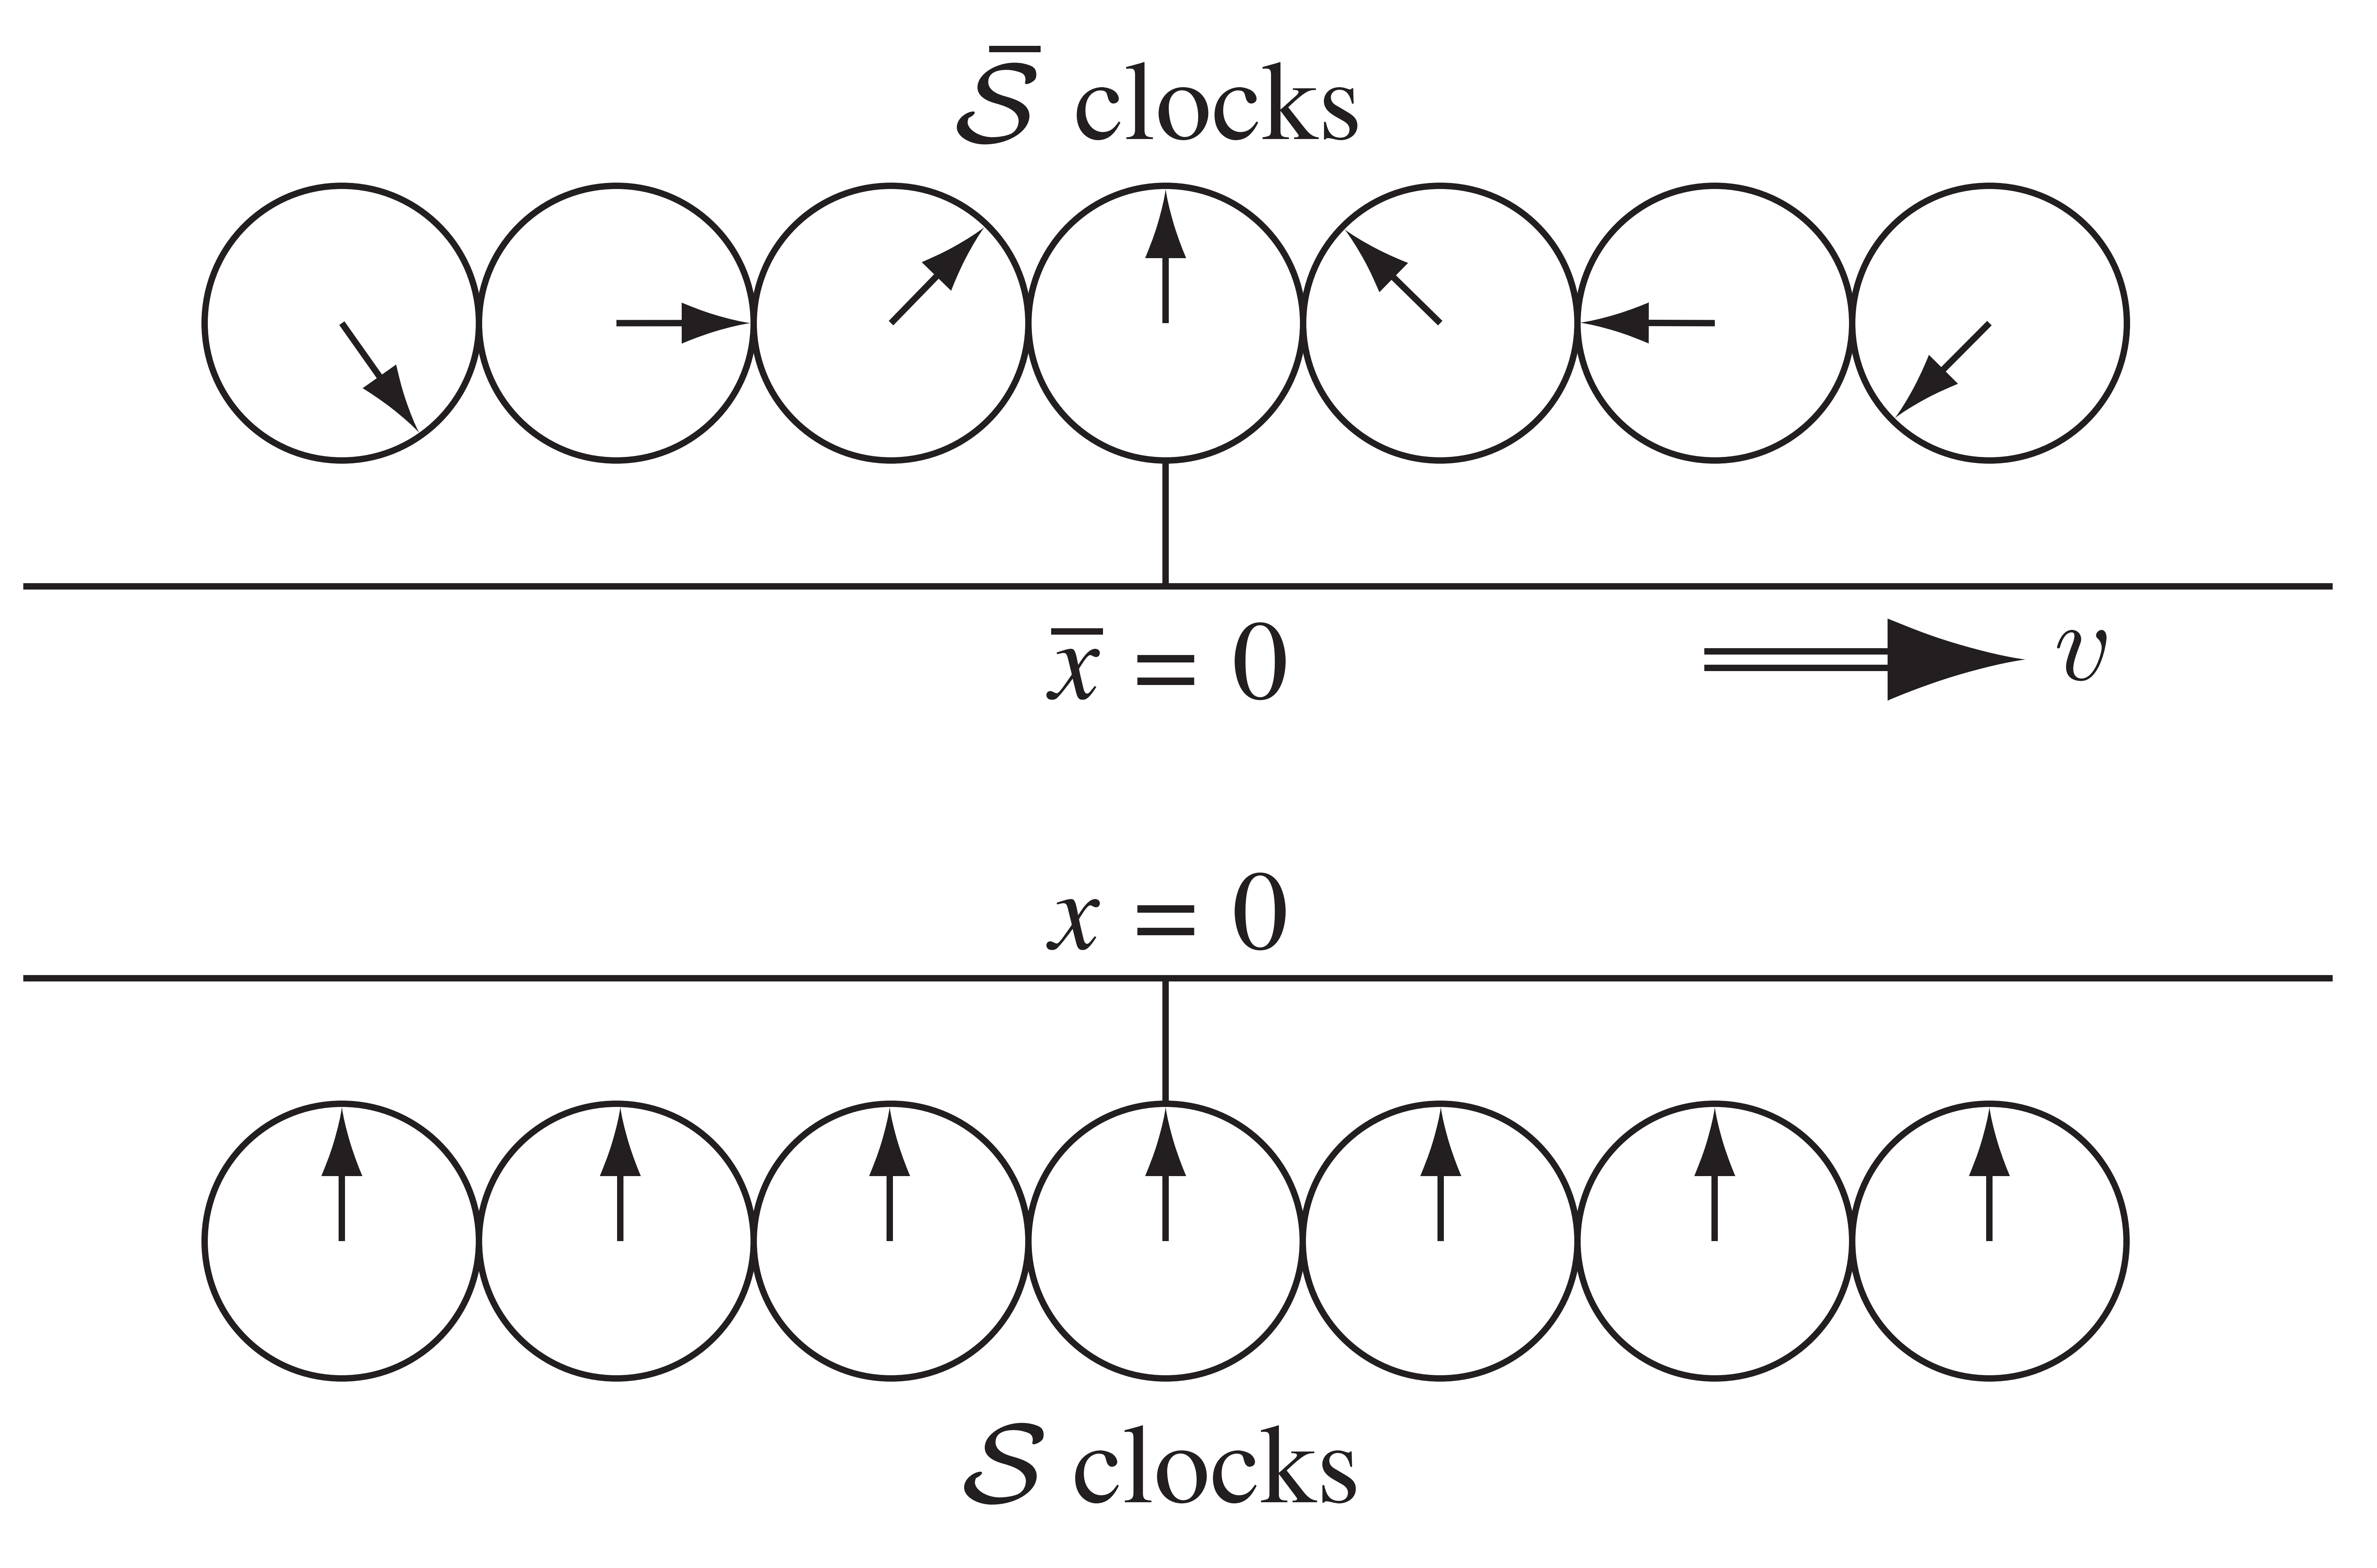
\includegraphics[height=4cm]{../Rss/Relativity/RelClocks.png}
    \caption*{Figure: Clocks that are properly synchronized in one system will not be synchronized when observed from another system}
\end{figure*}
Those to the left of the origin (negative x) are ahead, and those to the right are behind. $S$ focuses his attention on a single clock at rest in the $\bar{S}$ frame, and watches it over some interval $\Delta t$. Because $\bar{x}$ is fixed, the Reverse Lorentz transformations gives
\begin{equation*}
    \Delta \bar{t}=\frac{1}{\gamma}\Delta t
\end{equation*}

\textbf{Lorentz contraction.} To an observer on the train, the time it takes for light signal to be sent down and back 
\begin{equation*}
    \Delta \bar{t}=2\frac{\Delta \bar{x}}{c}
\end{equation*}
If $\Delta t_1$ is the time for the light signal to reach the front end, and $\Delta t_2$ is the return time, then to an observer on the ground
\begin{equation*}
    \Delta t_1=\frac{\Delta x+v\Delta t_1}{c}\qquad \Delta t_2=\frac{\Delta x-v\Delta t_2}{c}
\end{equation*}
\begin{figure*}[b]
    \centering
    
\includegraphics[width=\textwidth]{../Rss/Relativity/LorentzContraction.png}
    \caption*{Figure: Railway carriage, if you will}
\end{figure*}
solving for $\Delta t_1$ and $\Delta t_2$
\begin{equation*}
    \Delta t_1=\frac{\Delta x}{c-v}\qquad \Delta t_2=\frac{\Delta x}{c+v}
\end{equation*}
So the round-trip time is
\begin{equation*}
    \Delta t=2\frac{\Delta x}{c}\frac{1}{1-v^2/c^2}
\end{equation*}
Applying time dilation formula and solving for $\Delta x$
\begin{equation*}
    \Delta \bar{x}=\frac{1}{\sqrt{1-v^2/c^2}}\Delta x=\gamma \Delta x
\end{equation*}

Now, Imagine a stick at rest in $\bar{S}$. Its rest length is $\Delta \bar{x}$. If an observer in S were to measure the stick, he would subtract the positions of the two ends at one instant of his time $t$. In another word, t is fixed and Lorentz transformations give
\begin{equation*}
    \Delta \bar{x}=\gamma \Delta x
\end{equation*}

\textbf{Einstein's velocity addition rule.} Suppose a particle moves a distance $dx$ (in $S$) in a time $dt$. Its velocity $u$ is then
\begin{equation*}
    u=\frac{dx}{dt}
\end{equation*}
In $\bar{S}$, meanwhile, it has moved a distance
\begin{equation*}
    d\bar{x}=\gamma(dx-vdt)
\end{equation*}
in a time 
\begin{equation*}
    d\bar{t}=\gamma (dt-\frac{v}{c^2}dx)
\end{equation*}
The velocity in $\bar{S}$ is therefore
\begin{equation*}
    \bar{u}=\frac{d\bar{x}}{d\bar{t}}=\frac{u-c}{1-uv/c^2}
\end{equation*}
To recover the more transparent notation, let $A$ be the particle, $B$ be $S$, and $C$ be $\bar{S}$; then $u = v_{AB}$ , $\bar{u} = v_{AC}$, and $v = v_{C B} = -v_{BC}$, so 
\begin{equation*}
    v_{AC}=\frac{v_{AB}+v_{BC}}{1-+(v_{AB}v_{BC}/c^2)}
\end{equation*}

\subsection*{Structure of Spacetime}
\textbf{Four-vectors.} The Lorentz transformations take on a simpler appearance when expressed in terms of the quantities
\begin{equation*}
    x^0\equiv ct\qquad \beta\equiv \frac{v}{c}
\end{equation*}
If, at the same time, we number the $x$, $y$, $z$ coordinates, so that
\begin{equation*}
    x^1\equiv x\qquad x^2\equiv y\qquad x^3\equiv z
\end{equation*}
then the Lorentz transformations read
\begin{align*}
    \bar{x^0} &= \gamma (x^0 - \beta x^1)\\
    \bar{x^1} &= \gamma(x^1-\beta x^0)\\
    \bar{x^2} &= x^2\\
    \bar{x^3}&=x^3
\end{align*}
Or, in matrix form:
\begin{equation*}
    \begin{pmatrix}
        \bar{x^0}\\
        \bar{x^1}\\
        \bar{x^2}\\
        \bar{x^3}
    \end{pmatrix}=
    \begin{pmatrix}
        \gamma&-\gamma\beta&0&0\\
        -\gamma\beta&\gamma&0&0\\
        0&0&1&0\\
        0&0&0&1\\
    \end{pmatrix}
    \begin{pmatrix}
        {x^0}\\
        {x^1}\\
        {x^2}\\
        {x^3}
    \end{pmatrix}
\end{equation*}
Letting Greek indices run from 0 to 3, this can be distilled into a single equation:
\begin{equation*}
\bar{x}^{\mu}=\sum_{v=0}^{3}\Lambda_{v}^{\mu}x^v
\end{equation*}
where is $\Lambda$ the Lorentz transformation matrix in (the superscript $\mu$ labels the row, the subscript v labels the column). (3-d) vector defined as any set of three components that transform under rotations the same way (x, y, z) do; by extension, we now define a 4-vector as any set of four components that transform in the same manner as ($x_0$, $x_1$, $x_2$, $x_3$) under Lorentz transformations:
\begin{equation*}
\bar{a}^{\mu}=\sum_{v=0}^{3}\Lambda_{v}^{\mu}a^v
\end{equation*}

There is a 4-vector analog to the dot product, but it’s not just the sum of the products of like components; rather, the zeroth components have a minus sign
\begin{equation*}
\mathbf{A}\cdot\mathbf{B}=-a^0b^0+ a^1b^1+ a^2b^2+ a^3b^3
\end{equation*}
It has the same value in all inertial systems; just as the ordinary dot product is invariant (unchanged) under rotations, this combination is invariant under Lorentz transformations. 

It is convenient to introduce the covariant vector $a^\mu$, which differs from the contravariant $a^\mu$ only in the sign of the zeroth
\begin{equation*}
a^\mu= (a_0, a_1, a_2, a_3) \equiv (-a^0, a^1, a^2, a^3)
\end{equation*}
Upper indices designate contravariant vectors; lower indices are for covariant vectors. Raising or lowering the temporal index costs a minus sign; raising or lowering a spatial index changes nothing. Formally,
\begin{equation*}
    a_\mu=\sum_{v=0}^{3}g_{\mu v}a^v\qquad q\equiv
    \begin{pmatrix}
        -1&0&0&0\\
        0&1&0&0\\
        0&0&1&0\\
        0&0&0&1\\
    \end{pmatrix}
\end{equation*}
The scalar product can now be written with the summation symbol
\begin{equation*}
    \sum_{\mu=0}^{3}a^\mu b_\mu
\end{equation*}
or, more compactly still
\begin{equation*}
    a^\mu b_\mu
\end{equation*}
This is called the Einstein summation convention, after its inventor, who regarded it as one of his most important contributions. Of course, we could just as well take care of the minus sign by switching to covariant b
\begin{equation*}
    a^\mu b_\mu = a_\mu b^\mu = -a^0b^0 + a^1b^1 + a^2b^2 + a^3b^3
\end{equation*}

\textbf{The invariant interval.} The scalar product of a 4-vector with itself,
\begin{equation*}
    a^\mu a_\mu  = -(a^0)^2 + (a^1)^2 + (a^2)^2 + (a^3)^2 
\end{equation*}
can be positive (if the “spatial” terms dominate) or negative (if the “temporal” term dominates) or zero:
\begin{align*}
    \text{If}\qquad a^\mu a_\mu>0,\qquad a^\mu\quad\text{is called }\textbf{spacelike}\\
    \text{If}\qquad a^\mu a_\mu<0,\qquad a^\mu\quad\text{is called }\textbf{timelike}\\
    \text{If}\qquad a^\mu a_\mu=0,\qquad a^\mu\quad\text{is called }\textbf{lightlike}\\
\end{align*}
Suppose event A occurs at ($x_A^0$, $x_A^1$, $x_A^2$, $x_A^3$) and event B at ($x_B^0$, $x_B^1$, $x_B^2$, $x_B^3$). The difference
\begin{equation*}
    \Delta x^\mu\equiv x_A^\mu-x_B^\mu
\end{equation*}
is the displacement 4-vector. The scalar product of $\Delta x^\mu$ with itself is called the invariant interval between two events:
\begin{align*}
    I&\equiv (\Delta x)^\mu(\Delta x)_\mu= -(\Delta x^0)^2 + (\Delta x^1)^2 + (\Delta x^2)^2 + (\Delta x^3)^2 \\
    &=-c^2t^4+d^2
\end{align*}
If the displacement between two events is timelike ($I < 0$), there exists an inertial system (accessible by Lorentz transformation) in which they occur at the same point. On the other hand, if the displacement is spacelike ($I > 0$), then there exists a system in which the two events occur at the same time. And if the displacement is lightlike ($I = 0$), then the two events could be connected by a light signal.

\textbf{Space-time diagrams.} On such a Minkowski diagrams, position plotted horizontally and time (or, better, $x^0 = ct$) vertically. Velocity is then given by the reciprocal of the slope. A particle at rest is represented by a vertical line; a photon, traveling at the speed of light, is described by a 45◦ line; and a rocket going at some intermediate speed follows a line of slope $c/v = 1/\beta$.
\begin{figure*}
    \centering
    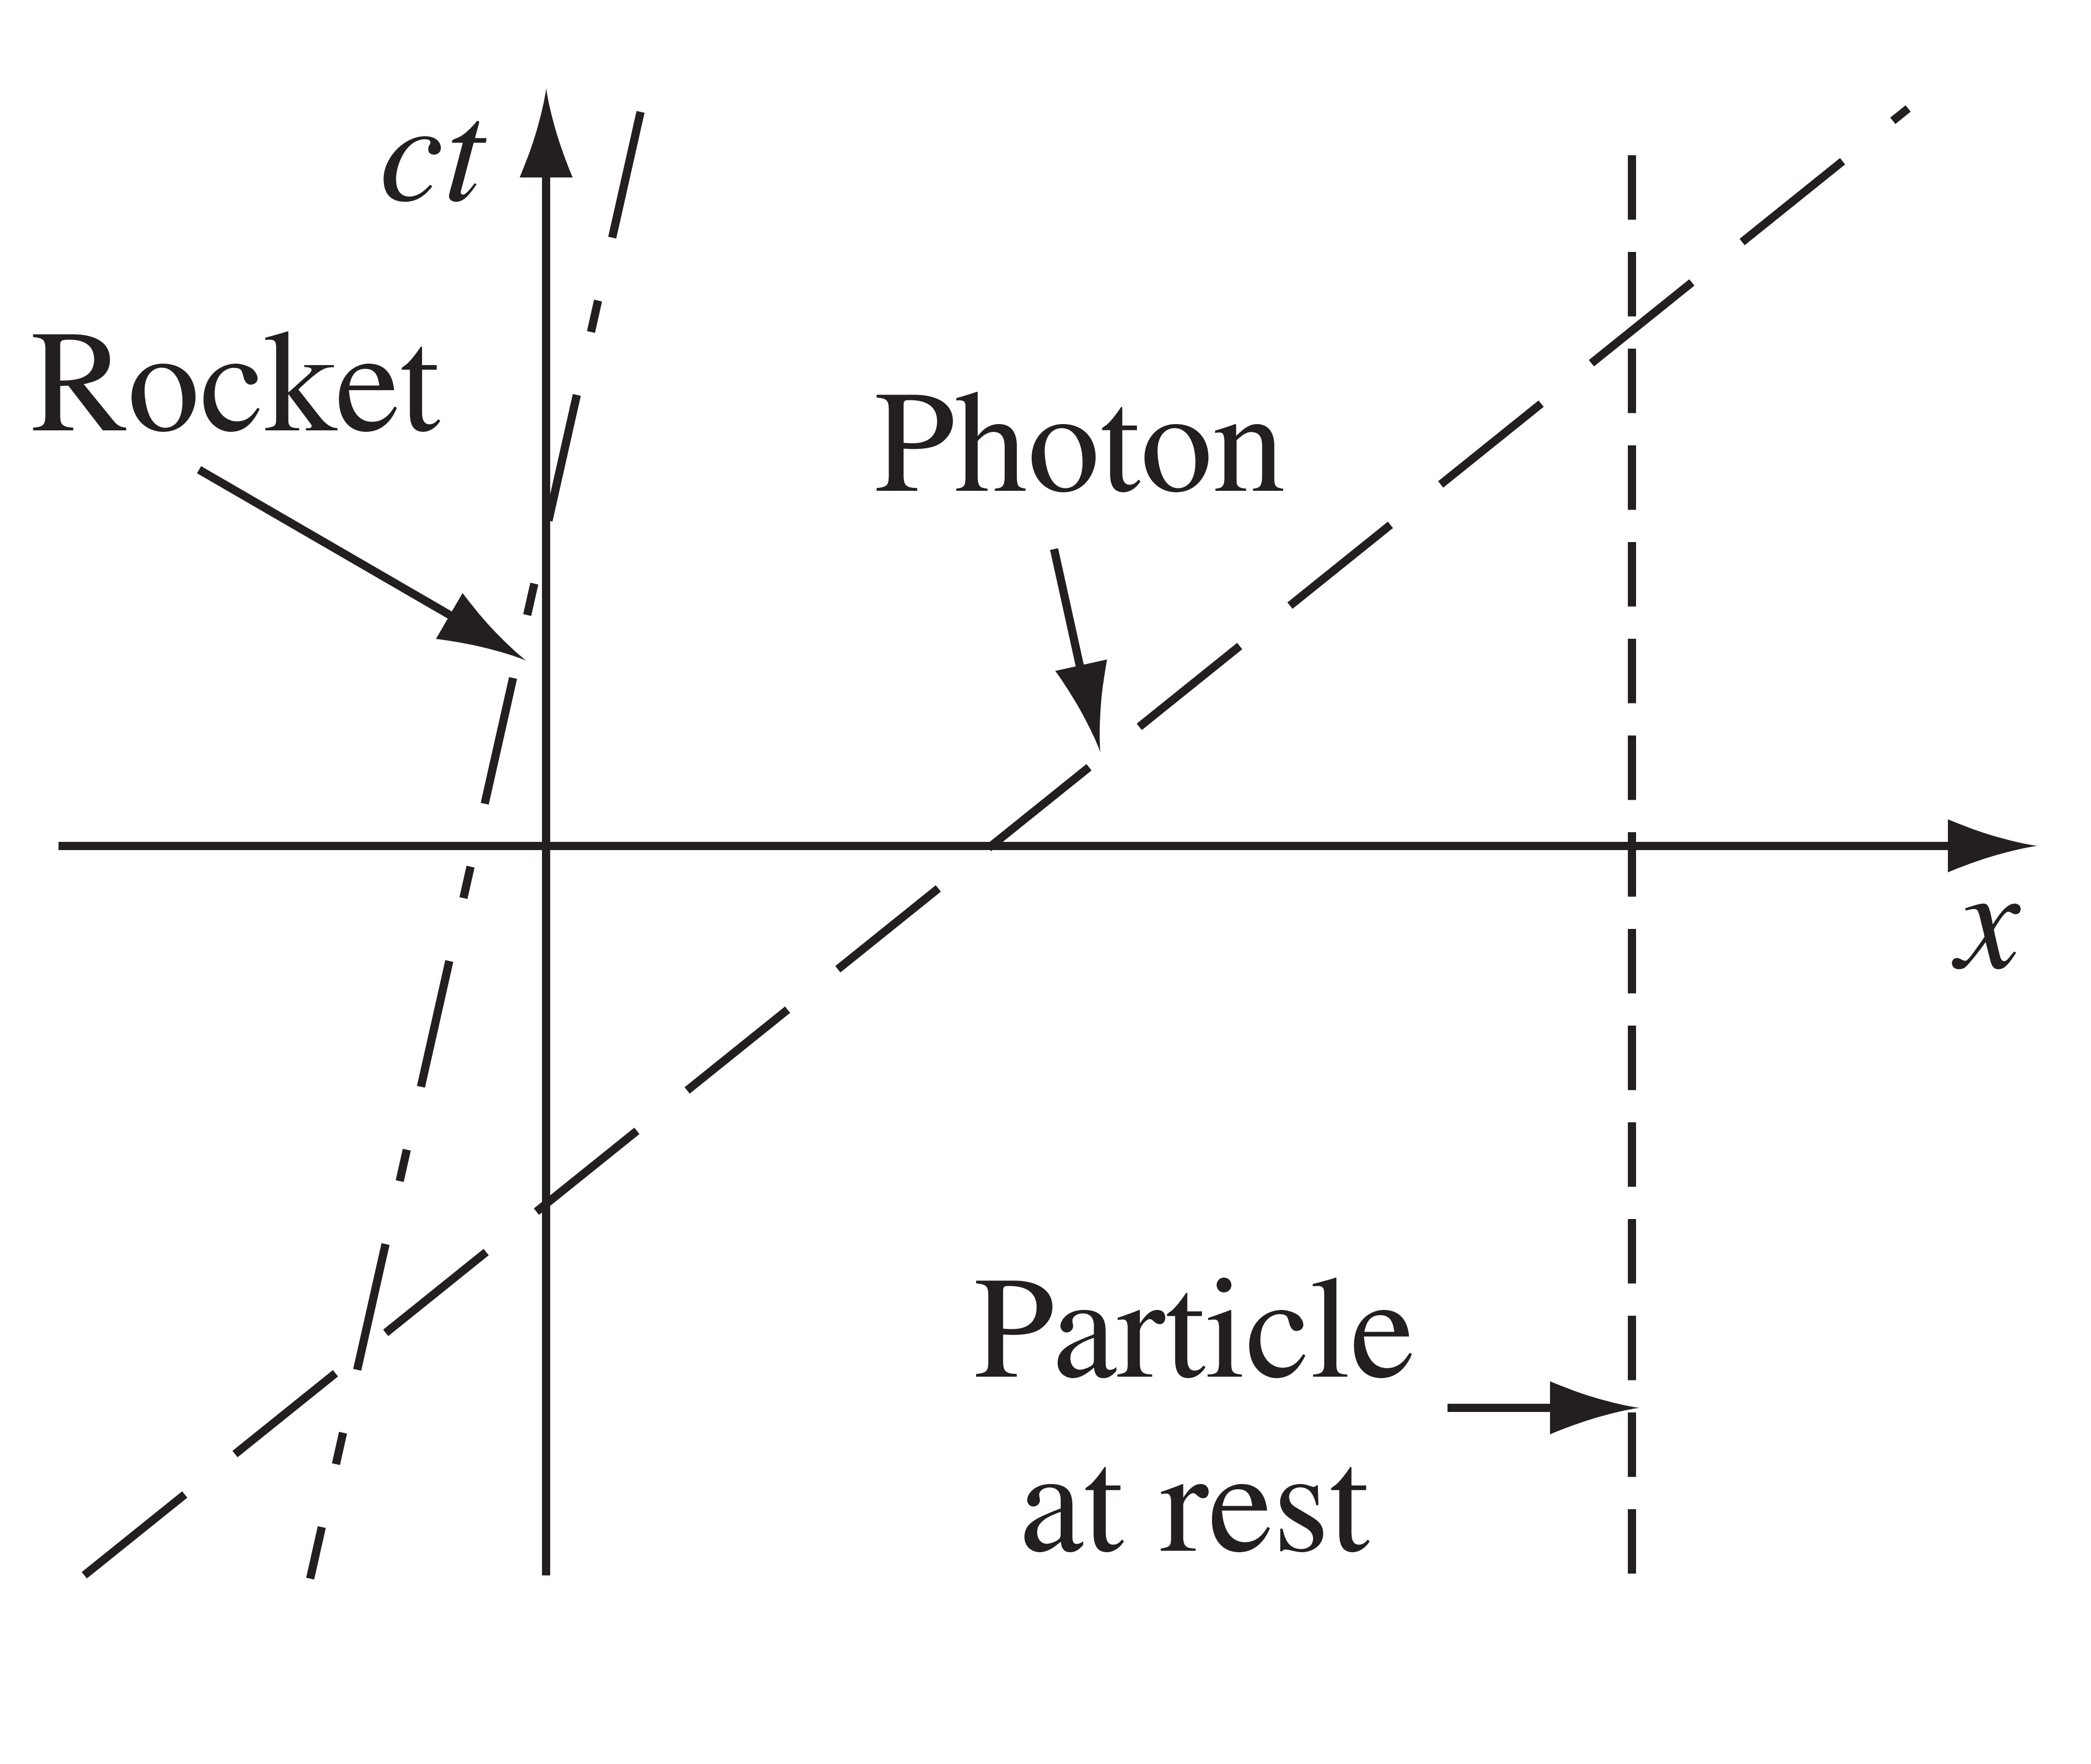
\includegraphics[height=4cm]{../Rss/Relativity/MinkowskiDig.png}
    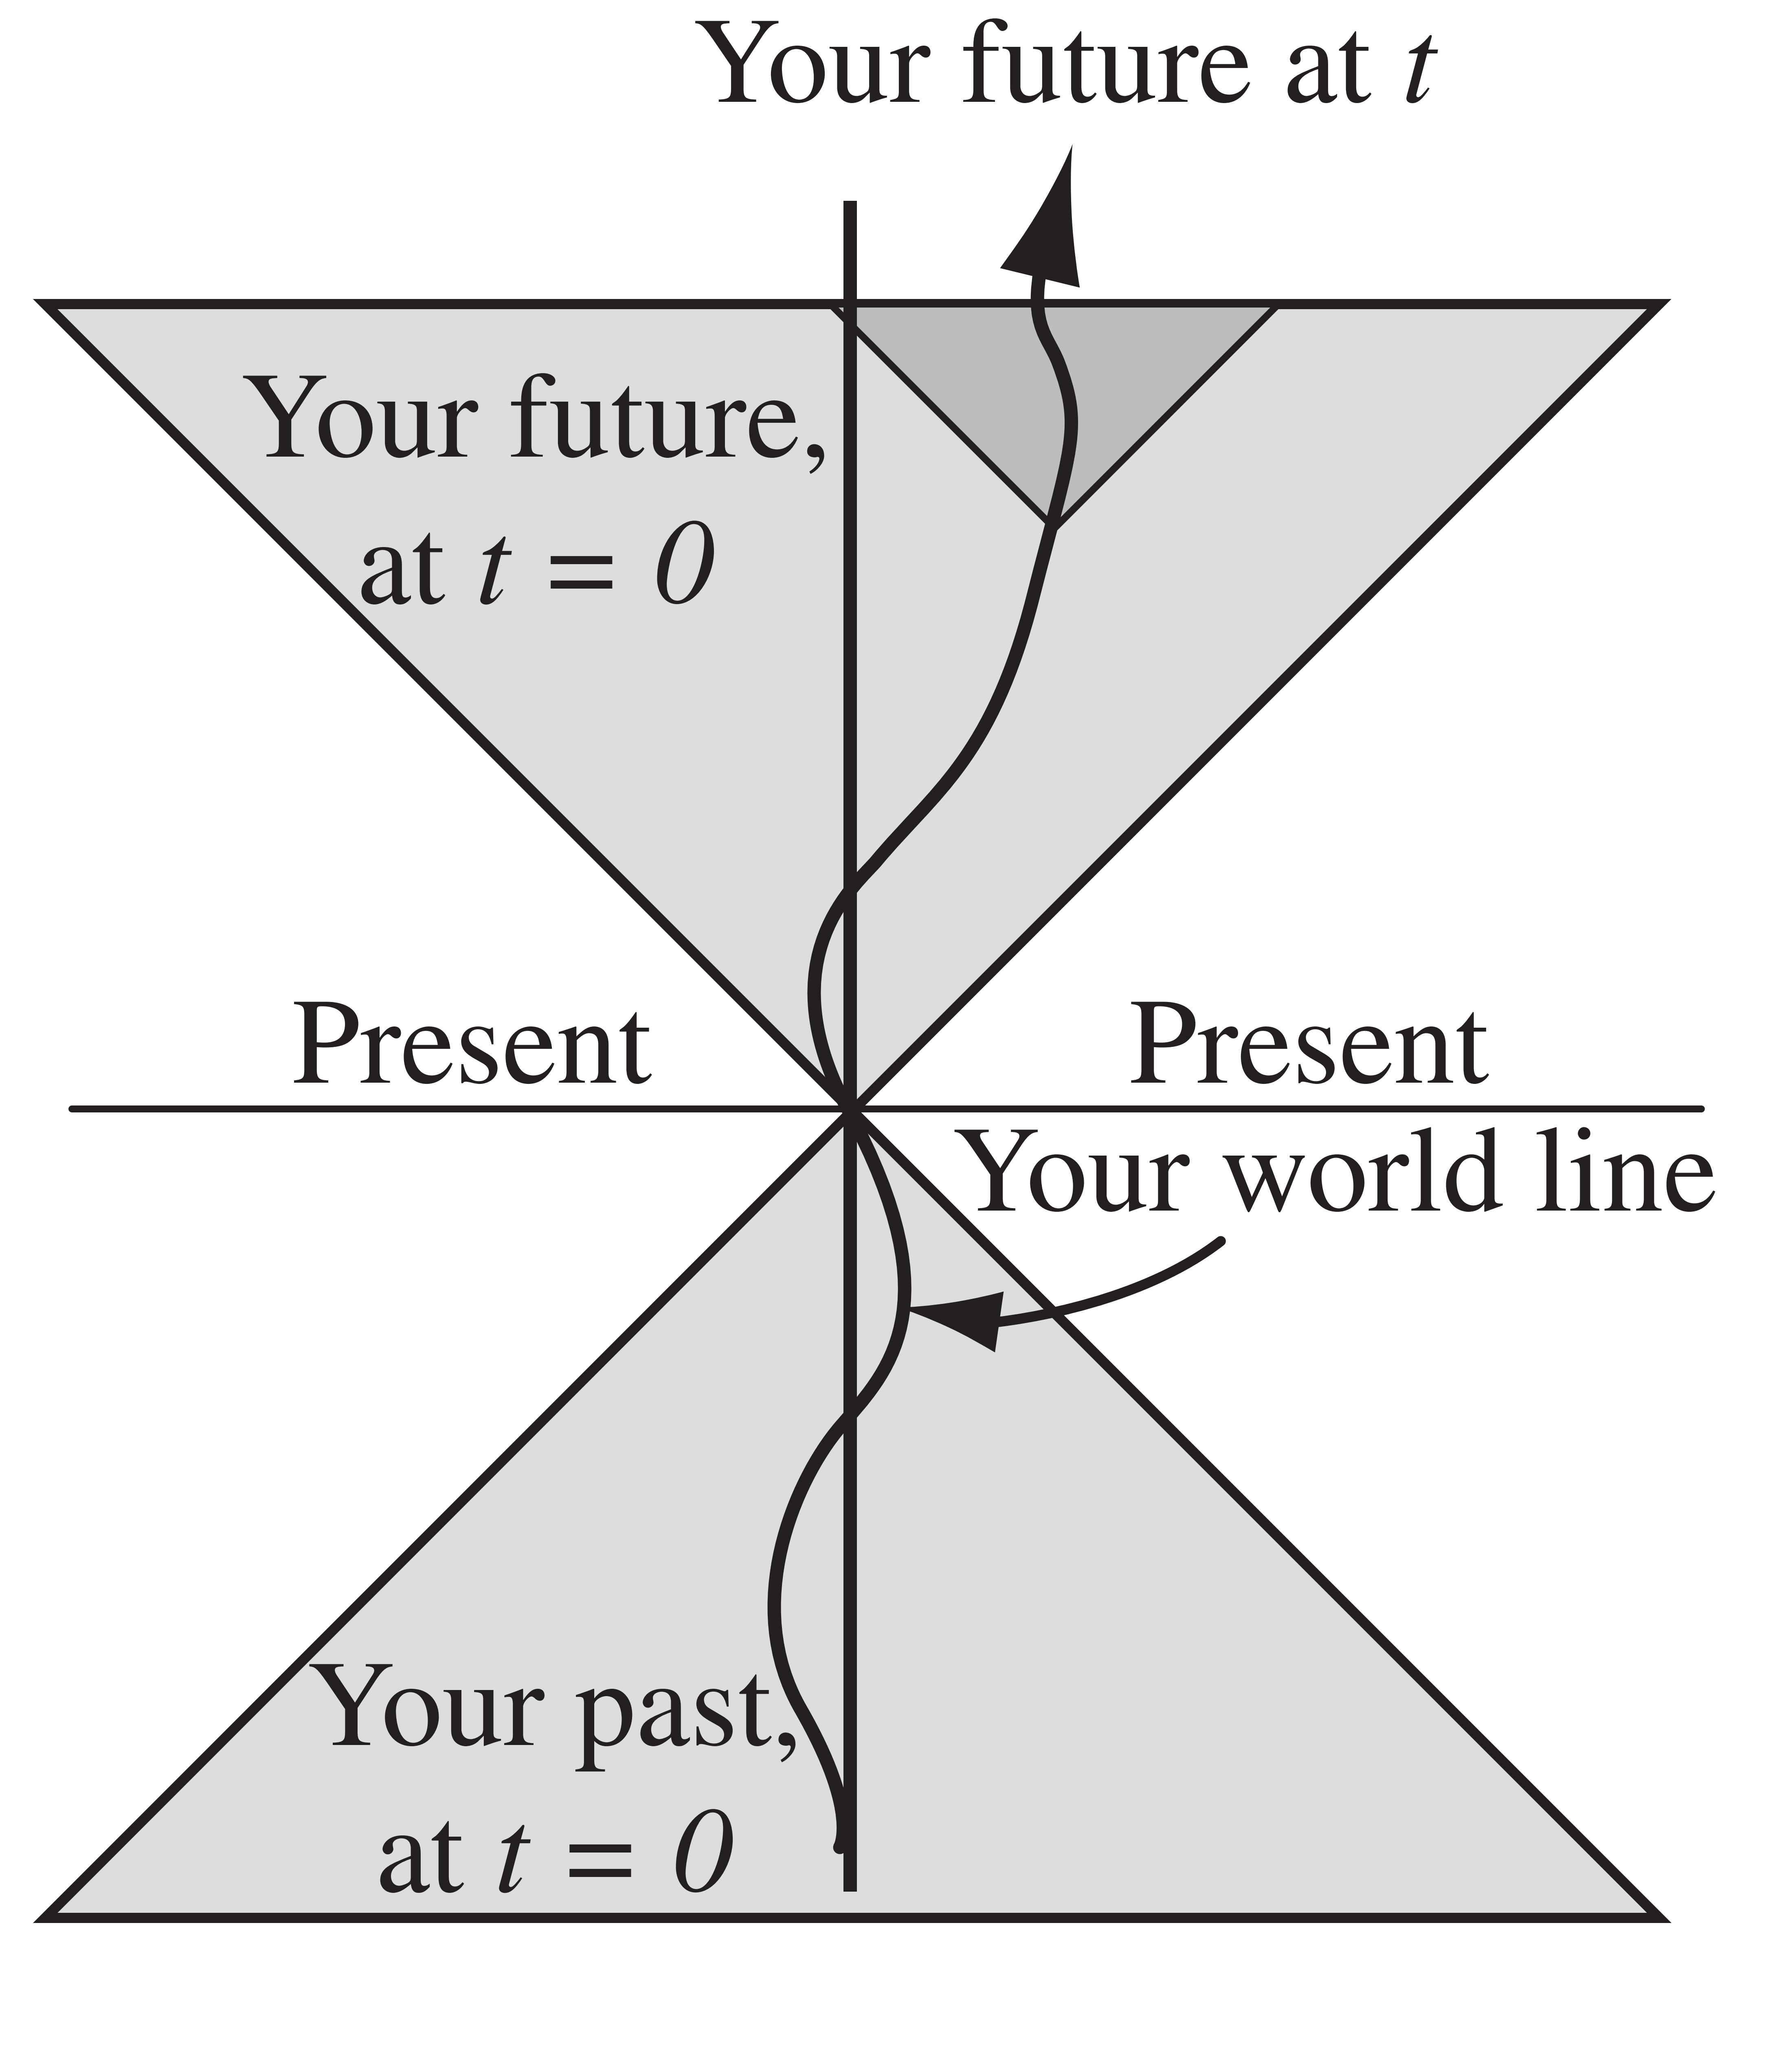
\includegraphics[height=4cm]{../Rss/Relativity/WorldLine.png}
    \caption*{Figure: Minkowski diagrams}
\end{figure*}

The trajectory of a particle on a Minkowski diagram is called a world line. Because no material object can travel faster than light, your world line can never have a slope less than 1. Accordingly, your motion is restricted to the wedge-shaped region bounded by the two 45\textdegree lines. We call this your “future,” in the sense that it is the locus of all points accessible to you. as time goes on, and you move along your chosen world line, your options progressively narrow. Meanwhile, the backward wedge represents your “past,” in the sense that it is the locus of all points from which you might have come. As for the rest, this is the generalized “present.” There's no way you can influence any event in the present; it's a vast expanse of spacetime that is absolutely inaccessible to you. If we include a y axis coming out of the page, the “wedges” become cones—and, with an undrawable z axis, hypercones. Because their boundaries are the trajectories of light rays, we call them the forward light cone and the backward light cone. Your future, in other words, lies within your forward light cone, your past within your backward light cone.

Under Lorentz transformations, the interval $I$ is preserved, and the locus of all points with a given value of I is a hyperbola—or, if we include the y axis, a hyperboloid of revolution. When the displacement is timelike, it's a “hyperboloid of two sheets”; when the displacement is spacelike, it's a “hyperboloid of one sheet.” When you perform a Lorentz transformation, the coordinates ($x$, $t$) of a given event will change to ( $\bar{x}$, $\bar{t}$), but these new coordinates will lie on the same hyperbola as (x, t). No amount of transformation will carry it, say, from the upper sheet of the timelike hyperboloid to the lower sheet, or to a spacelike hyperboloid.
\begin{figure*}
    \centering
    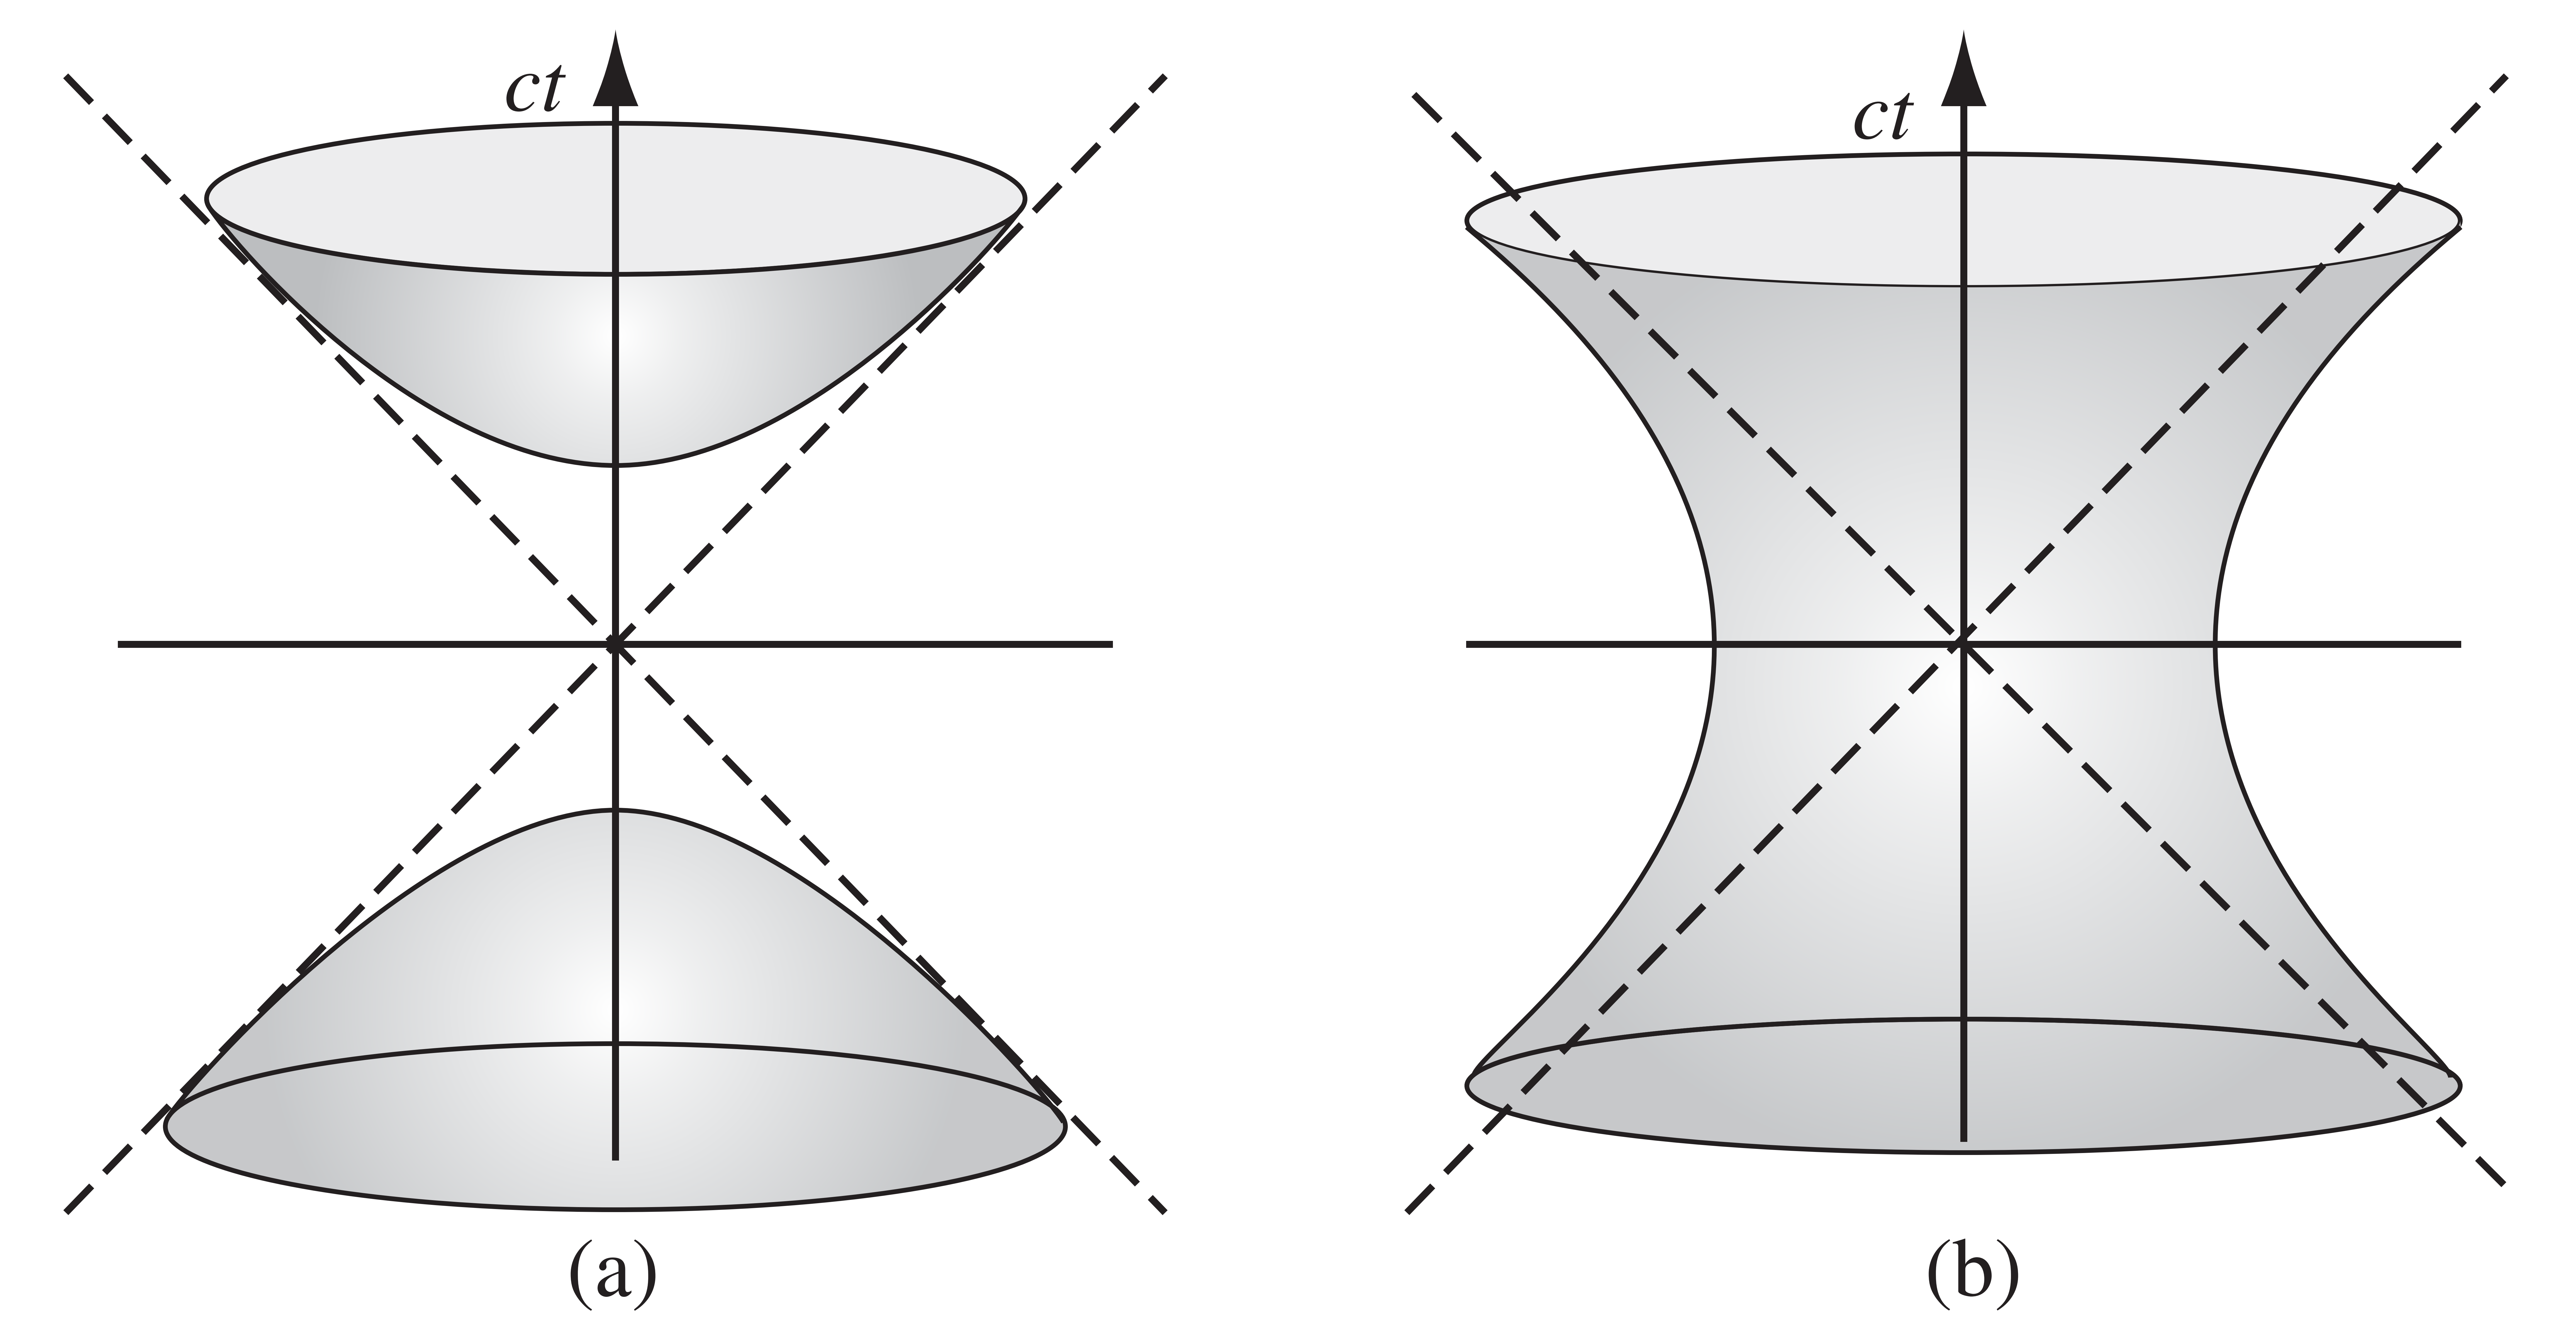
\includegraphics[height=4cm]{../Rss/Relativity/Hypercones.png}
    \caption*{Figure: Hypercones}
\end{figure*}

If the displacement 4-vector between two events is timelike, their ordering is absolute; if the interval is spacelike, their ordering depends on the inertial system from which they are observed. In terms of the space-time diagram, an event on the upper sheet of a timelike hyperboloid definitely occurred after (0, 0), and one on the lower sheet certainly occurred before; but an event on a spacelike hyperboloid occurred at positive t, or negative t, depending on your reference frame. Conclusion: The displacement between causally related events is always timelike, and their temporal ordering is the same for all inertial observers.

Here's some neat summary
\begin{center}
        \begin{longtable}{ |p{0.3\textwidth}|p{0.3\textwidth} |p{0.3\textwidth}| }
            \hline
            Timelike separation&Spacelike separation&Lightlike separation\\
            \hline
            $I < 0$&$I > 0$&$I = 0$\\
            $a^\mu a_\mu<0$&$a^\mu a_\mu>0$&$a^\mu a_\mu=0$\\
            The two events may or may not have a causal connection.&The two events cannot have a causal
            connection.&The two events may or may not have a causal connection.(citation needed!)\\
            All observers will agree about the order in which the two events occurred.&Different observers will disagree about the order in which the two events occurred.&Different observers will disagree about the distance between them and the time between them, but everyone will agree that the distance equals the time multiplied by c.\\
            There will be one reference frame in which the two events happened at the same place.&There will be one reference frame in which the two events happened at the same time.&(source incomplete!)\\
            \hline
        \end{longtable}
\end{center}

\subsection*{Proper Time and Proper Velocity}
As you progress along your world line, your watch runs slow; while the clock on the wall ticks off an interval $dt$, your watch only advances $d\tau$:
\begin{equation*}
    d\tau=\sqrt{1 - u^2/c^2}dt
\end{equation*}
The time $\tau$ your watch registers (or, more generally, the time associated with the moving object) is called proper time. I'll use u for the velocity of a particular object--you, in this instance--and reserve v for the relative velocity of two inertial systems.  The velocity
\begin{equation*}
    \mathbf{u}=\frac{d\mathbf{l}}{dt}
\end{equation*}
relative to ground (displacement divided by the time), both $d\mathbf{l}$ and $dt$ are to be measured by the ground observer.  However there is also distance covered per unit proper time
\begin{equation*}
    \boldsymbol{\eta}\equiv \frac{d\mathbf{l}}{d\tau}
\end{equation*}
This hybrid quantity (distance measured on the ground, over time measured by \emph{you}) is called proper velocity. 
\begin{equation*}
    \boldsymbol{\eta}= \frac{1}{\sqrt{1 - u^2/c^2}}\mathbf{u}
\end{equation*}
$\eta$ is the spatial part of a 4-vector
\begin{equation*}
    \eta\equiv\frac{dx^{\mu}}{d\tau}
\end{equation*}
whose zeroth component is
\begin{equation*}
    \eta^0=\frac{dx^{0}}{d\tau}=\frac{d}{d\tau}ct=\frac{c}{\sqrt{1 - u^2/c^2}}
\end{equation*}
Thus, for instance, when you go from system $S$ to system $\bar{S}$, moving at speed $v$ along the common $x\bar{x}$ axis,
\begin{align*}
    \bar{\eta^0} &= \gamma (\eta^0 - \beta \eta^1)\\
    \bar{\eta^1} &= \gamma(\eta^1-\beta \eta^0)\\
    \bar{\eta^2} &=\eta^2\\
    \bar{\eta^3}&=\eta^3
\end{align*}
More generally
\begin{equation*}
    \bar{\eta}^{\mu}=\Lambda_{v}^{\mu}\eta^v
\end{equation*}

$\eta^\mu$ is called the proper velocity 4-vector, or simply the 4-velocity. By contrast, the transformation rule for ordinary velocities \textbf{u} is quite cumbersome. The reason for the added complexity is plain: we're obliged to transform both the numerator $d\mathbf{l}$ and the denominator $dt$, whereas for proper velocity, the denominator $d\tau$ is invariant, so the ratio inherits the transformation rule of the numerator alone.
\begin{align*}
    \bar{u}_x=\frac{d\bar{x}}{d\bar{t}}=\frac{u_x-v}{1-vu_x/c^2}\\
    \bar{u}_y=\frac{d\bar{y}}{d\bar{t}}=\frac{u_y}{\gamma(1-vu_x/c^2)}\\
    \bar{u}_z=\frac{d\bar{z}}{d\bar{t}}=\frac{u_z}{\gamma(1-vu_x/c^2)}
\end{align*}

\textbf{Relativistic Energy and Momentum.} Relativistic momentum of an object of mass m traveling at (ordinary) velocity \textbf{u} 
\begin{equation*}
    p\equiv m\mathbf{\eta}=\frac{m\mathbf{u}}{\sqrt{1-u^2/c^2}}
\end{equation*}

Relativistic momentum is the spatial part of a 4-vector
\begin{equation*}
    p^\mu\equiv m\eta^\mu
\end{equation*}
with temporal component
\begin{equation*}
    p^0=\frac{mc}{\sqrt{1-u^2/c^2}}
\end{equation*}
Einstein identified $p^0c$ as relativistic energy
\begin{equation*}
    E\equiv\frac{mc^2}{\sqrt{1-u^2/c^2}}
\end{equation*}
Notice that the relativistic energy is nonzero even when the object is stationary; we call this rest energy:
\begin{equation*}
E_{\text{rest}}\equiv mc^2
\end{equation*}
The remainder, which is attributable to the motion, is kinetic energy
\begin{equation*}
E_{\text{kin}}\equiv E-mc^2=mc^2\bigg(\frac{1}{\sqrt{1-u^2/c^2}}-1\bigg)
\end{equation*}
So far, this is all just notation. The physics resides in the experimental fact:
\begin{quote}
    In every closed system, the total relativistic energy and momentum are conserved.
\end{quote}
Mass, however, is not conserved. Specifically , mass is invariant but not conserved; energy is conserved but not invariant; electric charge is both conserved and invariant; velocity is neither conserved nor invariant. Note the distinction between an invariant quantity (same value in all inertial systems) and a conserved quantity (same value before and after some process).

The scalar product of $p^\mu$ with itself is
\begin{equation*}
    p^\mu p_\mu=-(p^0)^2+(\mathbf{p}\cdot\mathbf{p})=-m^2c^2
\end{equation*}
In terms of the relativistic energy and momentum
\begin{equation*}
    E^2-p^2c^2=m^2c^4
\end{equation*}
For massless and relativistic particle
\begin{equation*}
    E=pc
\end{equation*}

\textbf{Michelson-Morley Experiment.} You alredy know the story of aether wind and how this experiment dissprove that model, so i'll omit that and focus on this experiment itself. The Michelson interferometer is represented in Figure \ref{fig:MMExperiment1}. Light from a single source reaches a half-silvered mirror and splits into two beams traveling at right angles to each other. The beams reach mirrors that send them back to the splitter, where they travel together to an eyepiece.
\begin{figure}
    \centering
    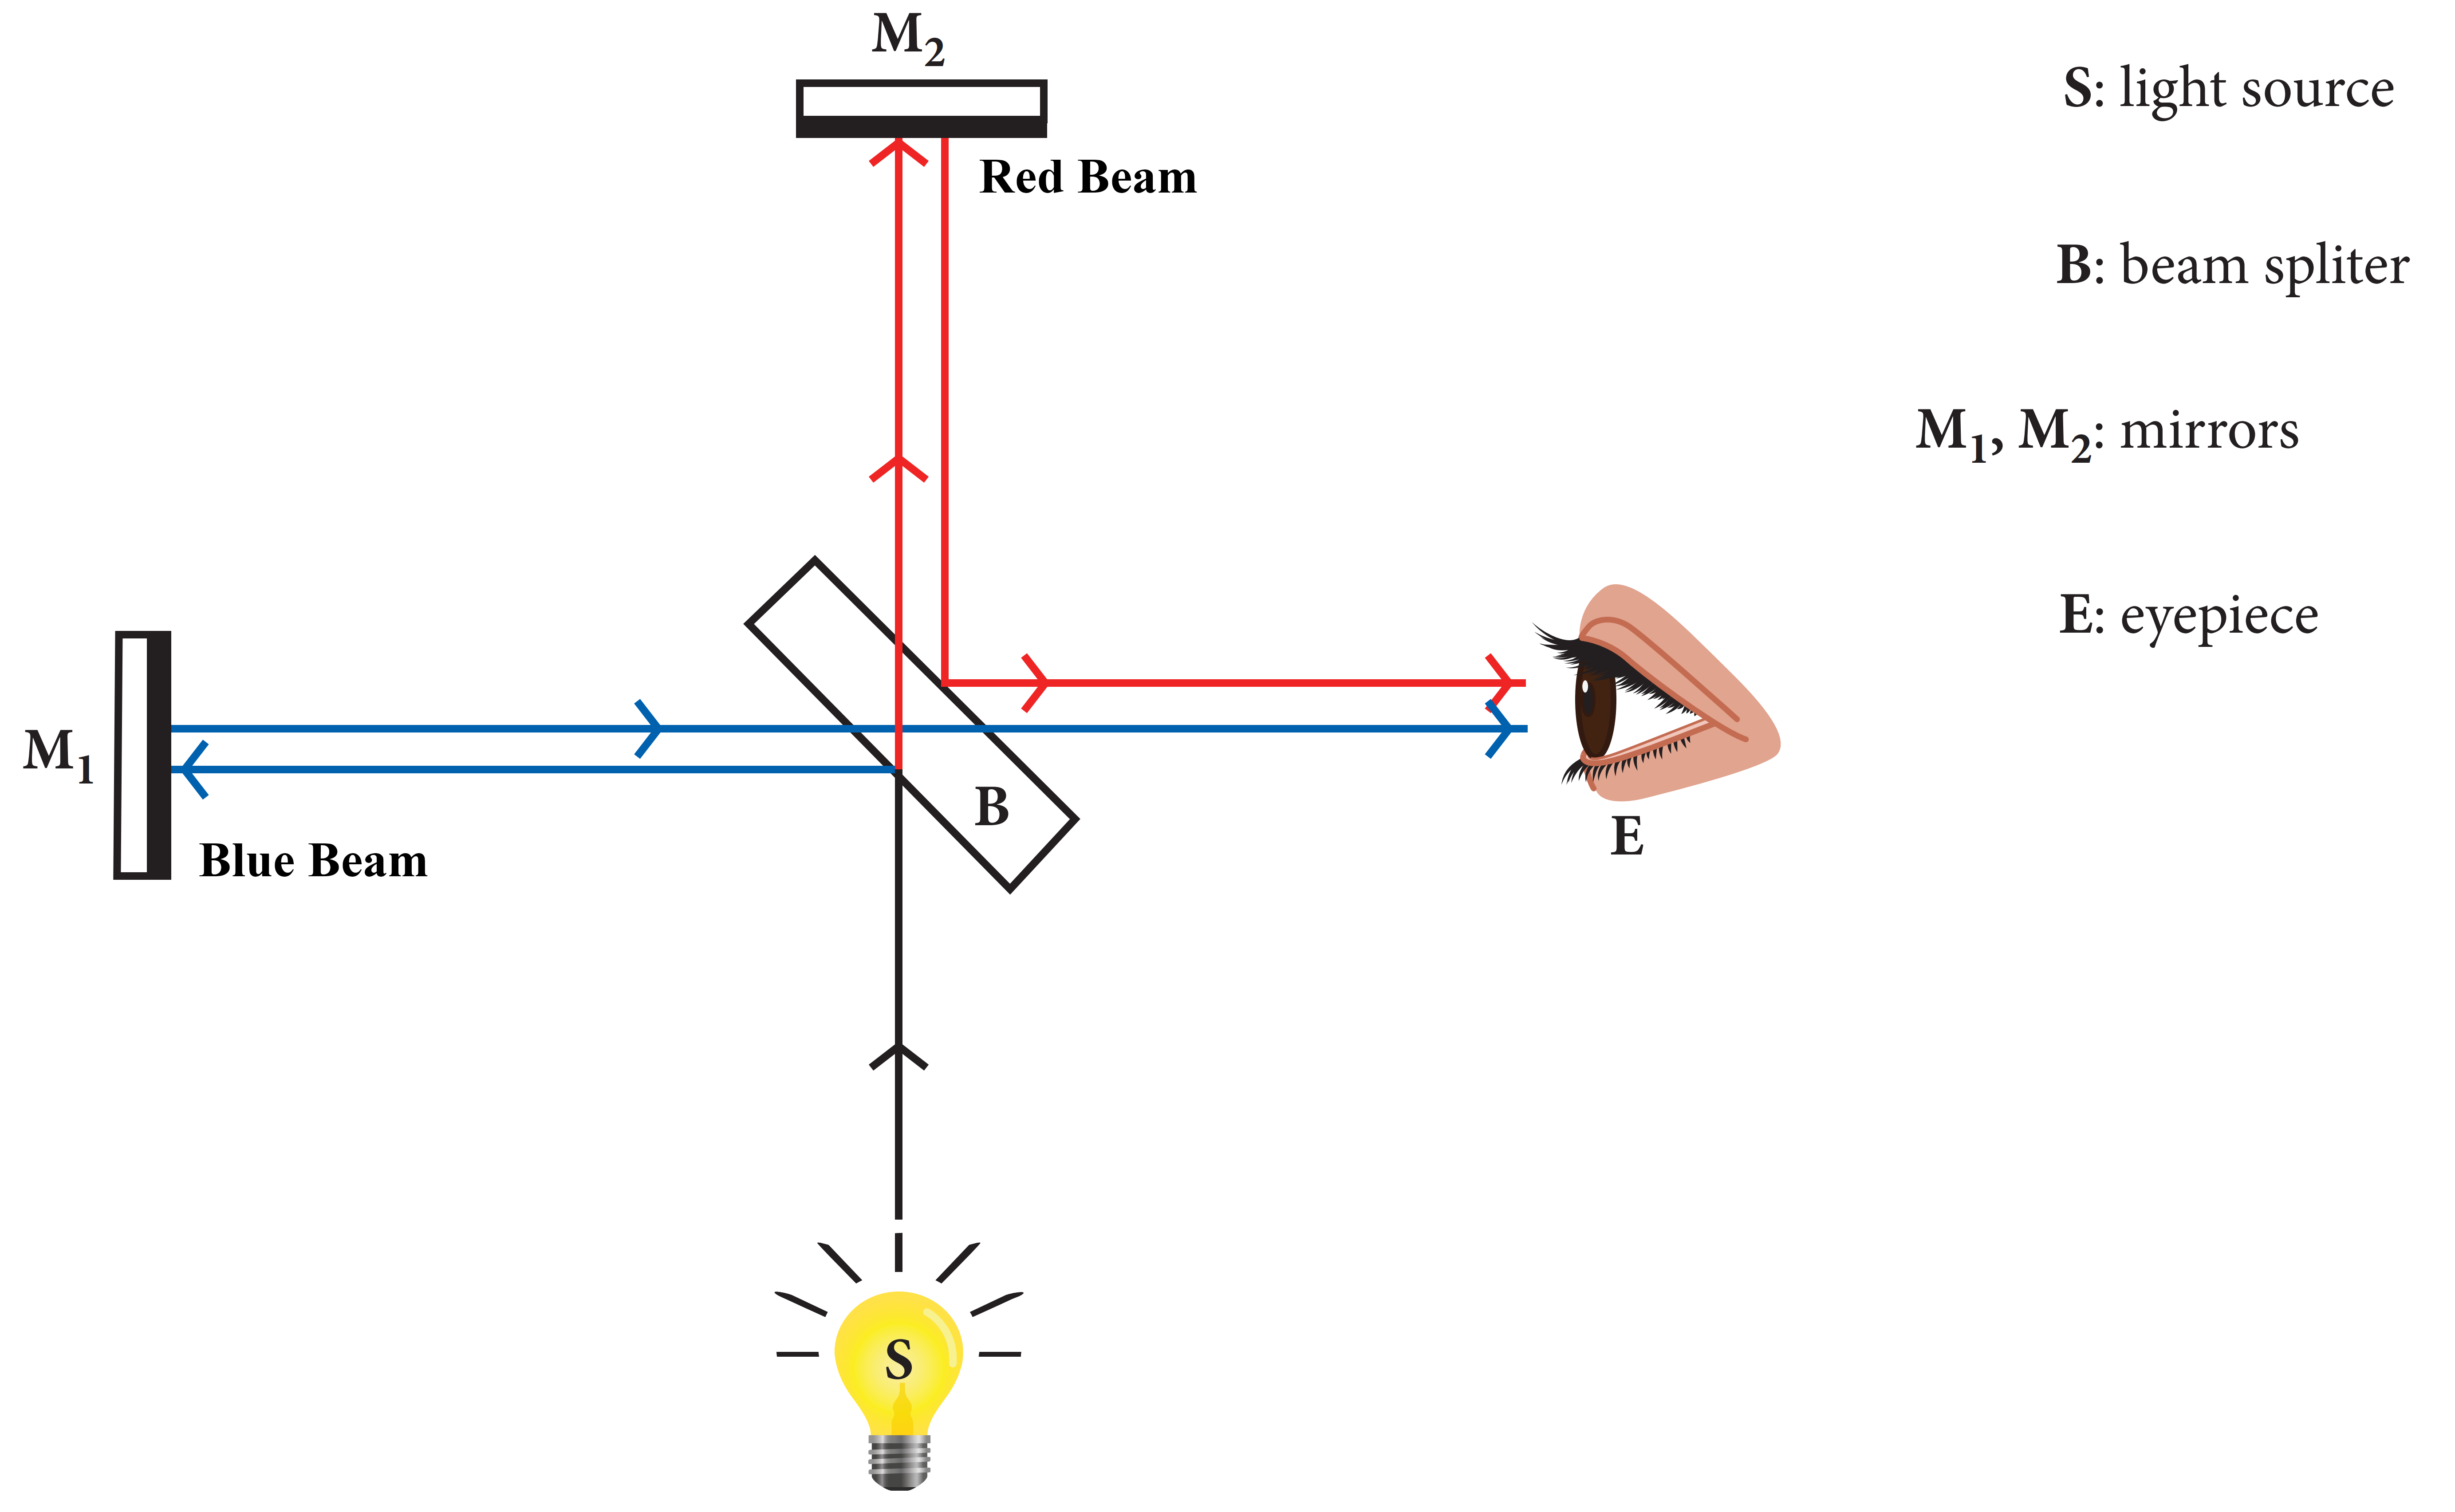
\includegraphics[height=4cm]{../Rss/Relativity/MichelsonMorley.png}
    \caption{Michelson-Morley Experiment}
    \label{fig:MMExperiment1}
\end{figure}
There are three possibilities that determine whether or not the two beams arrive in phase at the end of the eyepiece:
\begin{enumerate}
    \item If the two paths are identical in length, and the two beams travel identical speeds, then
    the two beams are in phase, and the interference is constructive.
    \item If the two paths are different lengths, then the beams may therefore arrive out of phase.
    \item If the two paths are identical lengths but are traveled at different speeds, then the two beams may be out of phase.
\end{enumerate}
Now suppose the Earth is traveling along the horizontal axis from $\mathbf{M}_1$ to \textbf{B}. The aether model predicts that for part of the trip the blue beam is going faster, and for part of the trip the red beam is going faster. But these two effects do not fully cancel out, and even if the two path lengths are identical, the beams will arrive out of phase.

After measuring the type of interference they observed, they rotated the entire apparatus. A uniform rotation does not change the geometry of the experiment; whatever phase change was caused by differences in path length is still exactly the same as it was. But a phase change caused by differences in speed, due to orientation with respect to the aether wind, will change. 

So the experiment was not to see whether the two beams constructively or destructively interfered on the wall, since such interference might have multiple causes. Rather, they looked to see how the interference pattern changed as they rotated the device. 

The result is, as you know it, their experiment found no evidence at all that the two beams had traveled at different speeds.  Michelson wrote in a letter that the result was “decidedly negative.” Even allowing for measurement errors, his experiment seemed to show that “the relative velocity [of the Earth and the aether] is less than one sixth of the Earth's velocity.”
\end{document}